\documentclass{mscLiterature}
\usepackage{subcaption}
\usepackage{wrapfig}
%
%
% Thesis data
%\mscDepartment{Delft Center for Systems and Control (\textsmaller{DCSC})}%
\mscProgram{Systems and Control}
%Change if needed to
%\mscProgram{Mechanical Engineering}
\mscFaculty{Mechanical, Maritime and Materials Engineering (3mE)}%
\mscName{B.J. van Hofslot}%
\mscDate{\today}%
\mscTitle{Humanoid Robot Locomotion Planning and Control}%
\mscSubTitle{Exploring the Effects of Center of Mass Height Variation}%
\mscKeyWords{thesis, msc, subject}% only used in PDF properties
\mscCoverPicture{STYLESTUFF/COVER}% to place a picture ( here the example COVER.eps) on the back of the cover page
\mscDepartment{Cognitive Robotics}
%
%
% Third party options (create text/logo on the copywrite page)
\mscThirdPartyText{The work in this survey was supported by the Institute for Human and Machine Cognition. Their cooperation is hereby gratefully acknowledged.}
\mscThirdPartyLogo{STYLESTUFF/EXAMPLELOGO}
% NOTE: on the title page only the TU Delft logo is permitted.
%
%
%
% Finalize the thesis data
\setThesisInfo
%
% Use \includeonly{} to build only certain parts of your thesis
%\includeonly{introduction, real_chapter, empty_chapter, long_chapter}%
%
%PH Toegevoegd 24-10-2011
%allow (matlab) listing max 1pt flexibility between lines
\lstset{lineskip=0pt plus 1pt minus 0pt}
%
\begin{document}
%
%========================== Front matter ======================================
\frontmatter %
%
% Make the cover page and hell of a lot of title pages
\maketitle
%
%
% Abstract (does not appear in the Table of Contents)
\chapter*{Abstract}%

This research considers using \ac{CoM} height variation as an input for balance control on a humanoid robot. Traditional balance strategies for humanoid robots are taking a step, control of the \ac{CoP} location, a result of the `ankle strategy', and changing the angular momentum about the \ac{CoM}, for example by a `hip strategy'. For humanoid robots, a common assumption behind these strategies is that the \ac{CoM} height is predefined. However, \ac{CoM} height changes can be used as an input for balance control, as for example can be observed during the landing of an athlete after a long jump. 

The first contributions of this work are bounds on the initial states for the \ac{VHIP} from which convergence is possible to a stopped state, also known as capture regions. First, only a unilateral contact constraint is considered; negative \ac{CoM} acceleration cannot be smaller than gravitational acceleration. Second, \ac{CoM} height constraints are added to the model, after which a capture region can still be computed in closed-form. Third, vertical force constraints are added, after which capture regions are computed numerically using a bang-bang control law. The last capture region bridges the transition to the applied part of this work.

The second contribution is a control law on vertical acceleration, suitable for application on a humanoid robot using a momentum-based control framework. Push recovery is tested on NASA's Valkyrie humanoid robot while the robot is standing. In simulation, an increase in recoverable push of $9$\% can be observed when comparing to a controller that only uses \ac{CoP}, when pushing the back of the robot. On hardware, an average increase of $7$\% can be observed for this push direction using a load sensor. Additionally, tests are conducted on hardware on Boston Dynamics' Atlas using a medicine ball on a rope, but no improvement in recovery is observed. The control method for standing push recovery is also extended for use while the robot is walking. For Valkyrie in simulation, recovery improved the most compared with a predefined height approach for a push applied in the first part of the single support state for rear and frontal push directions. Additionally, a hardware result on Atlas while walking is briefly presented.
%
% table of contents, (\toc of \toclof of \tocloflot )
\toclof
%
%
%%
% Preface
\chapter{Preface}

According to \textsc{WikipediA}, a preface (pronounced ``\emph{preffus}'') is an introduction to a book written by the author of the book. In this preface I can discuss the interesting story of how this thesis came into being. 

This is document is a part of my Master of Science graduation thesis. The idea of doing my thesis on this subject came after a discussion with my good friends Tweedledum and Tweedledee\ldots


%%
% Acknowledgements
\chapter{Preface \& Acknowledgments}%
Having a background in mechanical engineering, I have always been motivated in closing the gap between theory and application on a physical system during my master's in control systems. The topic of humanoid robotics offers a very interesting, challenging, platform to dedicate my motivation to. The complex multi-body system of a humanoid robot copes with nonlinearity, hybrid dynamics, actuation limitations and plays with your personal intuition. Also, humanoid robots are still physically far behind of what a human can do, which proves that there is large room for improvement. I believe in the future, substitution of a human with a human-like machine can be a live saving. I believe reaching out to \ac{IHMC} was the best decision to learn from and contribute to this field of research.

I would like to thank \ac{IHMC}, for giving me the opportunity to conduct research at the robotics lab. I am particularly grateful for the supervision that was given to me by Dr. Robert Griffin, Dr. Sylvain Bertrand and Dr. Jerry Pratt. I would like to thank everybody else at the robotics lab for their advice and the joy I experienced of working at the lab. 

I would also like to thank Dr. Javier Alonso-Mora from Delft University of Technology, for supervising me throughout the year I was abroad. Also, I would like to thank the examining committee members Prof. Dr. Martijn Wisse, Committee Member 4 and Committee Member 5.

I would like to thank my mother, father and two brothers, for always being supportive.

\vspace*{15mm}

Delft, University of Technology \hfill \mscname \\
\mscdate
%%
% Dedication page. 
\cleardoublepage
\thispagestyle{empty}
\vspace*{\stretch{1}}

% Put your own motto here, or dedicate your work to your Mom or whatever...
\begin{quote}
\noindent``Playing soccer is very simple, but the hardest thing there is, is playing soccer in a simple way.''
	
--- \emph{Johan Cruyff}
\end{quote}

\vspace{\stretch{3}}
\clearemptydoublepage
%
%========================== Main matter ======================================
\mainmatter
%
%
% Introduction
\chapter{Introduction} \label{chap::intro}%
There exist many situations in the world which are not safe, where a human is sent to help. Exploring the terrains of nuclear disasters, searching in a house on fire and clearing mine fields are all examples of this. Technology has extended the human's hand through history to a point where nowadays some people are wondering if we have almost hit the limits of fishing Mother Nature's pond of technology.  Safety standards in both professional and personal environments have greatly improved with the help of knowledge and technology. As is noticeable from the videos of Boston Dynamics going viral all over the world, legged robots, and more specifically humanoid robots, become more in a developed stage. However, comparing with the human physical capabilities, humanoid robots are still at most in a child phase.  The usefulness of these devices and the growth opportunities are a clear motivation to improve them.
\section{Motivation}
The walking humanoid robot system is highly complex. It deals with nonlinear multibody dynamics, complex kinematics, hybrid dynamics between switching ground contacts, unilateral friction-limited contact constraints and actuation limitations. Past research has approached nonlinearities with a linearized description of a walking robot \cite{kajita1992dynamic, pratt2006capture, koolen2012capturability} and has tackled joint level complexities by separating high level and joint level control \cite{kuindersma2016optimization, koolen2016design}. The planning problem of a walking gait has often been tackled by separating the footstep plan from the body motion plan \cite{chestnutt2005footstep,deits2014footstep,englsberger2014trajectory}. Although all these methods break the complexity of the system down and give a better approximation of how it will behave dynamically, often still a lot of assumptions are made. Linearization of the model has the advantage of giving a relatively simple measure, that can have a closed form solution in planning problems and that can be used in linear control. In Figure \ref{fig:3dlipfootinertiaz0} the basic model that is often considered is shown. The robot is modeled as a \ac{LIP} with constant height, were the foot and body inertia can be used for control. Recently research has been done in taking the constant height assumption away \cite{hopkins2014humanoid,liu2015trajectory, koolen2016balance, gao2017increase,nguyen2017dynamic, caron2018capturability}, but application of varying height models in control and planning is not yet proven to be successful. 
\section{Objective}
In this literature survey, the focus is to find how \ac{CoM} height variations are used in dynamic planning and control of a bipedal robot, with the goal of improving the dynamical behavior over rough, but also flat, terrain and improving robustness properties against disturbances. \\
Publications are compared based on several aspects. The needed underlying planning and control strategies for the presented methods play an important role, as they are related to the possibilities of application. The differences between \ac{2D} and \ac{3D} based methods can be pointed out and the differences between methods that require a predefined footstep plan and step timing in contrast to methods that define those. Computation times of the methods are compared, as they play an important role in real-time use. Presented results can be evaluated on the contribution to theory and application, where improvements or differences with respect to existing approaches are pointed out. In the case of control, robustness properties of the discussed strategy can be considered. As an example, strategies that fit a predefined footstep plan and that are presented in \ac{3D} are more likely to be applicable than a \ac{2D} strategy that defines the footsteps by the method itself, as most humanoids require a predefined footstep plan and rely on \ac{3D} dynamical models. \\
Even though the research area of focus is exploring the effects of varying height, a global study is done on humanoid robotics research in general, as it is important to understand which strategies are used in aspects that are related to the problem. \\
In Chapter \ref{chap:modeling}, a brief overview is given of basic humanoid walking related models and terminology. In Chapter \ref{chap:planningcontrol}, a general review is conducted on the current planning, control and state estimation strategies in humanoid robotics. Special attention is given to papers that were applied to Boston Dynamics' Atlas or NASA's Valkyrie at IHMC, as research is conducted and hopefully applied at this institute. In Chapter \ref{chap:varyingheight}, a full in-depth study is performed on publications that address \ac{CoM} height variation directly. In Chapter \ref{chap:conclusion}, a conclusion is made on the literature study and a goal for the research project is formulated. Information and ideas from different publications are tied together to attempt to formulate a balanced insight in the possibilities and concerns to tackle the problem.
\begin{figure}[h]
\centering
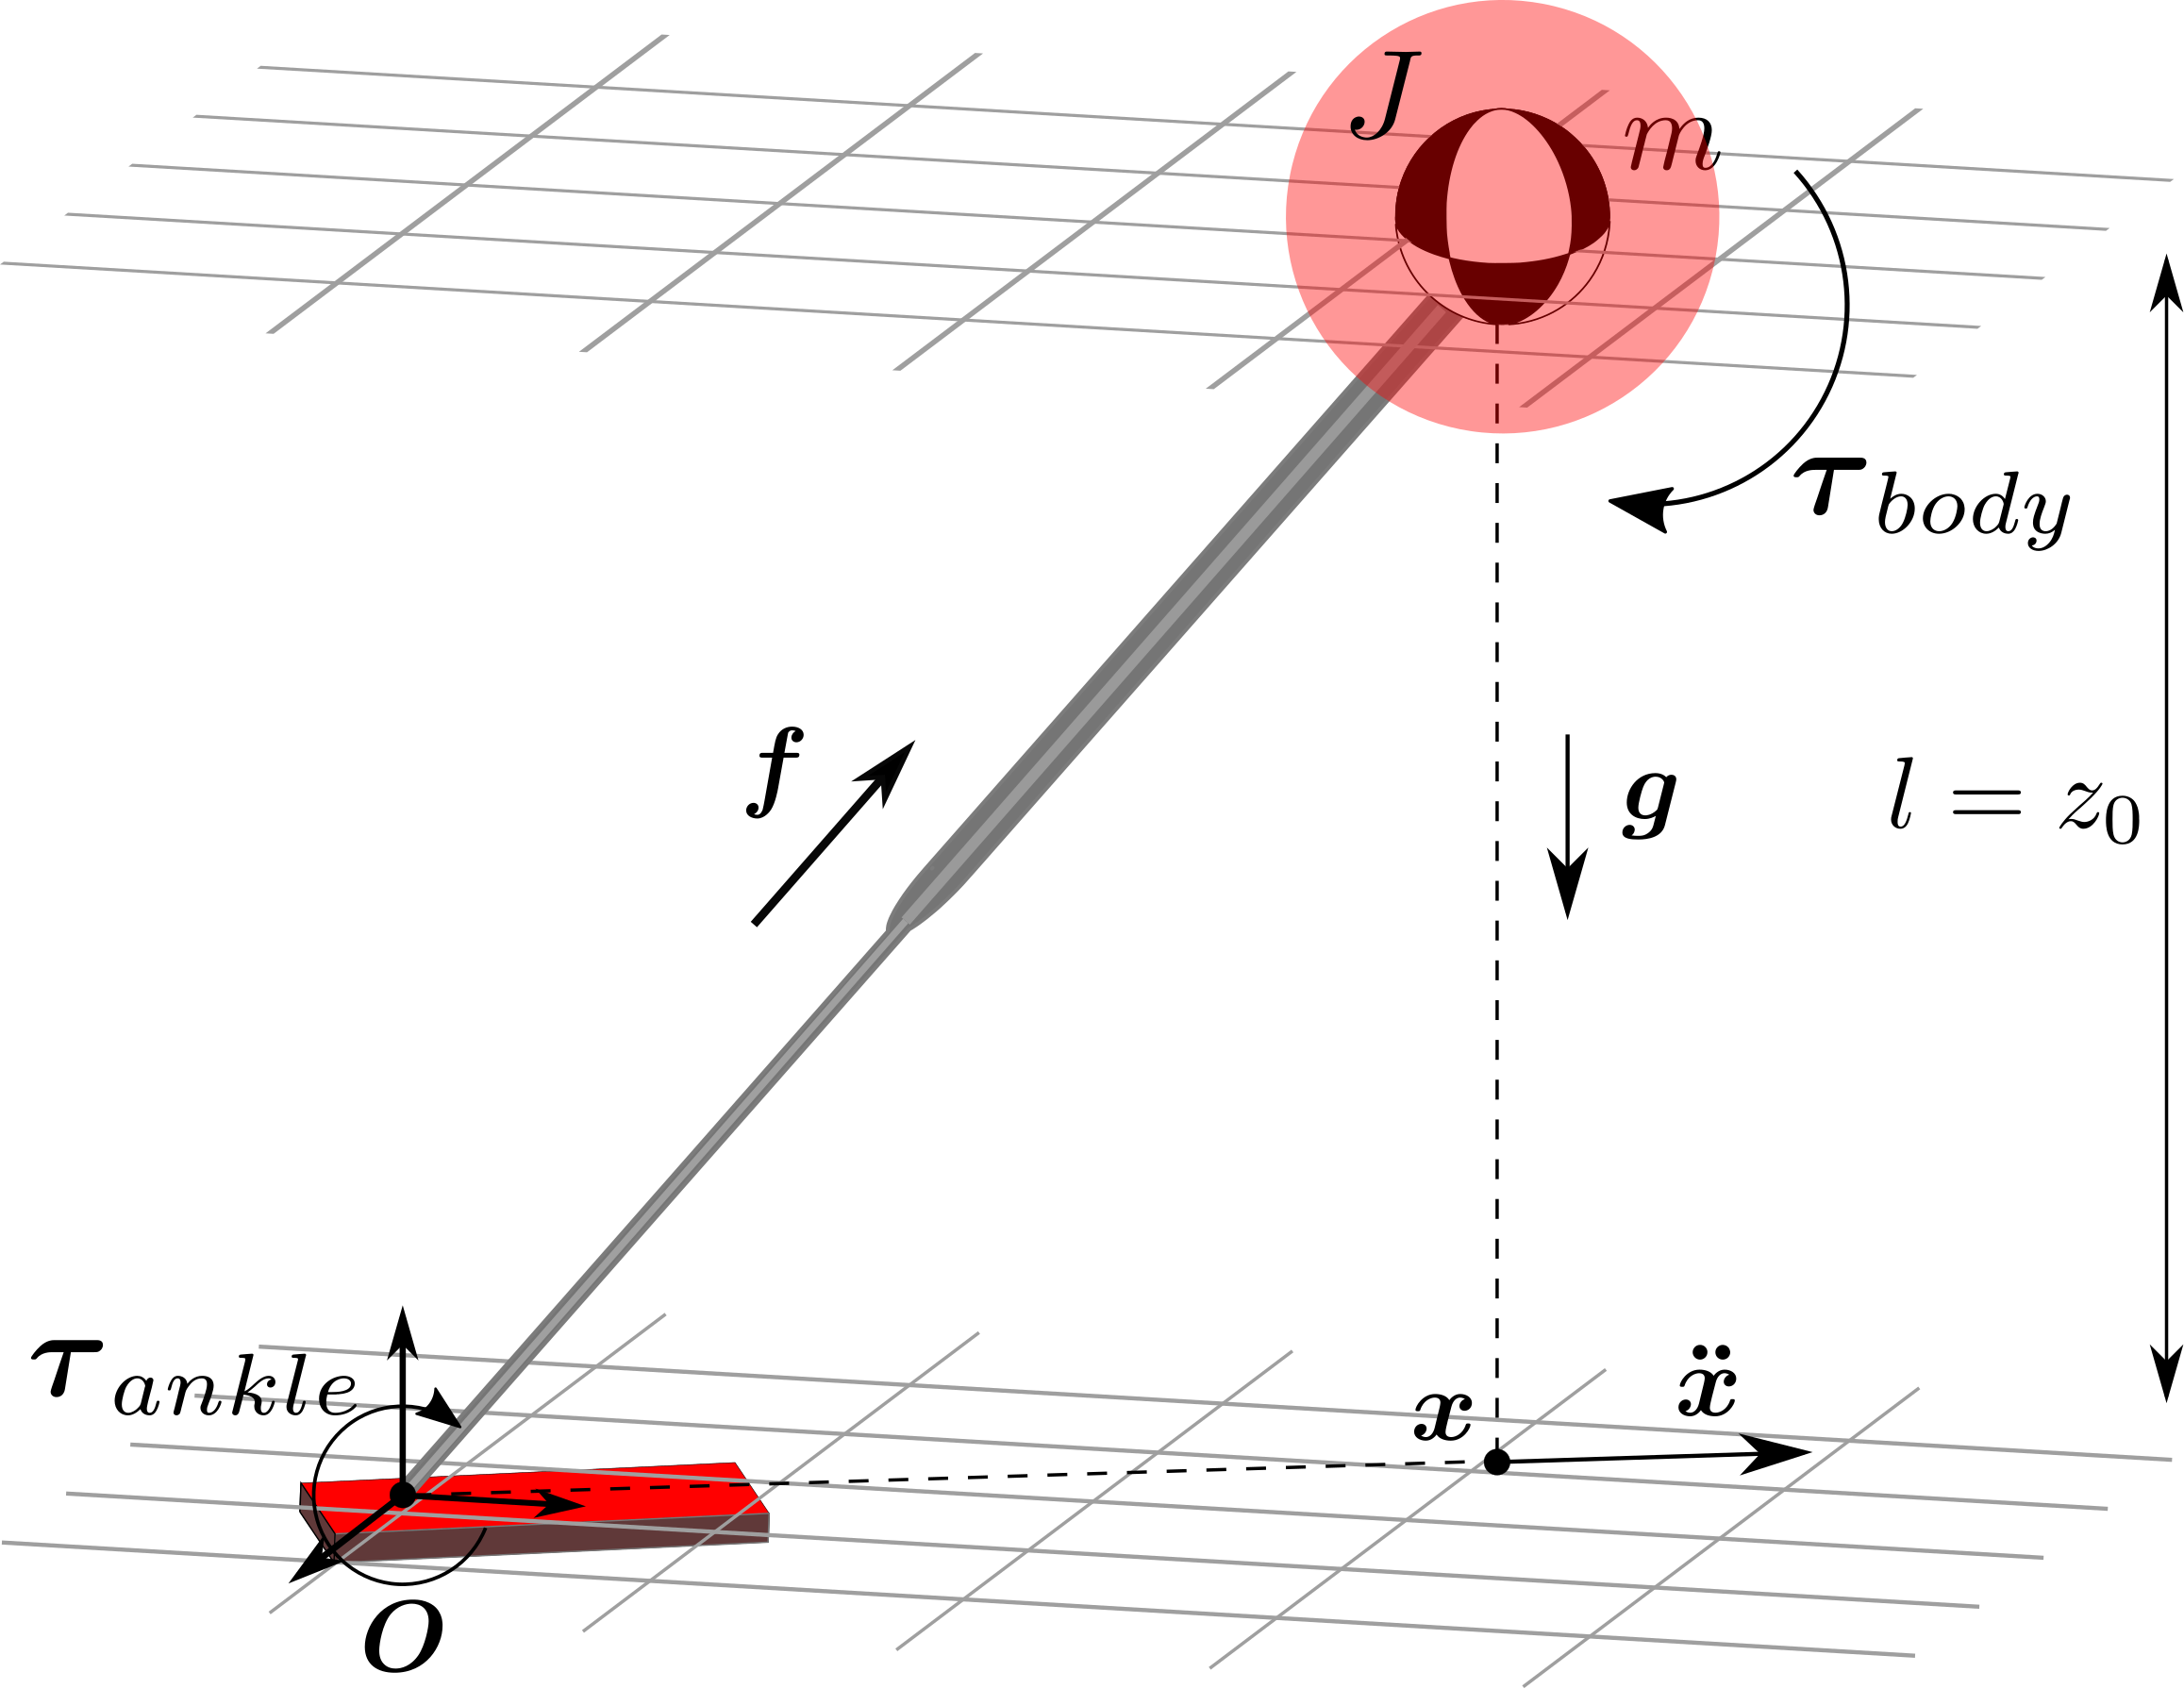
\includegraphics[width=0.5\textwidth]{STYLESTUFF/3DCoMfootinertiaz0.png}
\caption{\ac{3D} motion of \ac{LIP} model with foot at the base and a mass with inertia at the tip. The \ac{CoM} moves at constant height.}
\label{fig:3dlipfootinertiaz0}
\end{figure}





%
\chapter{Modeling \& Terminology}%
\label{chap:modeling}
As the design of humanoid robots is based on that of a human being, a lot of terms and models used by roboticists and human motion researchers overlap.  In this chapter, an overview is given of an important part of the fundamental naming and theory that is used for the system behavior and description of a humanoid robot. 
\section{Walking Terminology}
There are a variety of terms used in describing walking or locomotion. In this section, the terminology in this report is determined, which is also widely used, as for example can be found in \cite{charalambous2014walking}.
\subsection{Single support phase}
During the single support phase, the biped is only with one foot on the ground. The other foot is swinging through the air without ground contact, in the process of taking a step. The leg in contact with the ground is called the \textit{stance leg} and the leg taking a step is called the \textit{swing leg}. In a simplified walking model the single support phase with hybrid switching between contacts is often the only phase considered. There exist also bipedal robots with only this phase applied on hardware, like ATRIAS from Oregon State University \cite{ramezani2014performance}. This robot however, by the point-foot support with only the single stance leg per single support phase, has to keep stepping without interruption to stay stable, as the unstable equilibrium above the foot diverges quickly. 
\subsection{Double support phase}
In more human-like walking, next to the single support phase the double support phase is considered, also called the transfer phase in some cases. This is the phase during walking where both feet are on the ground.

\section{Full Robot Model}
The human body is a very complex system and has redundant joints and actuation. Among those joints exist joints with one degree of freedom, like the knee joint, but also joints with multiple degrees of freedom, like the hip joint for example. Reproducing this in robotics is a challenging task and different choices can be made in the complexity of the system and the type of actuators. 
\subsection{Current bipedal robots}
In \figref{fig:currentrobots} a couple of modern bipedal robots are displayed. \figref{fig:currentrobotsa} displays the newest model of Boston Dynamics' Atlas, a device that impressed a lot of people with its capabilities. It can run, stand up again after it has fallen over and it can even do a backflip, as shown in videos. Those are all incredible improvements with respect to earlier achieved results in humanoid robotics. \figref{fig:currentrobotsb} shows the previous Atlas model. This robot is used by IHMC to compete in the DARPA Robotics Challenge \cite{johnson2015team} and it gets still used to test new features on. \figref{fig:currentrobotsc} shows the Valkyrie humanoid robot \cite{radford2015valkyrie}, which is built by NASA. A version of this robot is also at IHMC. A difference between the Atlas robots and Valkyrie, is that the both Atlas versions are controlled with hydraulic actuation. Valkyrie makes use of so called series elastic actuators. \figref{fig:currentrobotsd} shows the ATRIAS robot from Oregon State University \cite{ramezani2014performance}. This is a good example of a, compared to the previous three examples, relatively more simple model. It has point feet and no arms for manipulation. In this report this is therefore defined as a bipedal robot, but not as a humanoid.
\begin{figure}[h]
  \begin{subfigure}{0.23\textwidth}
  \centering
  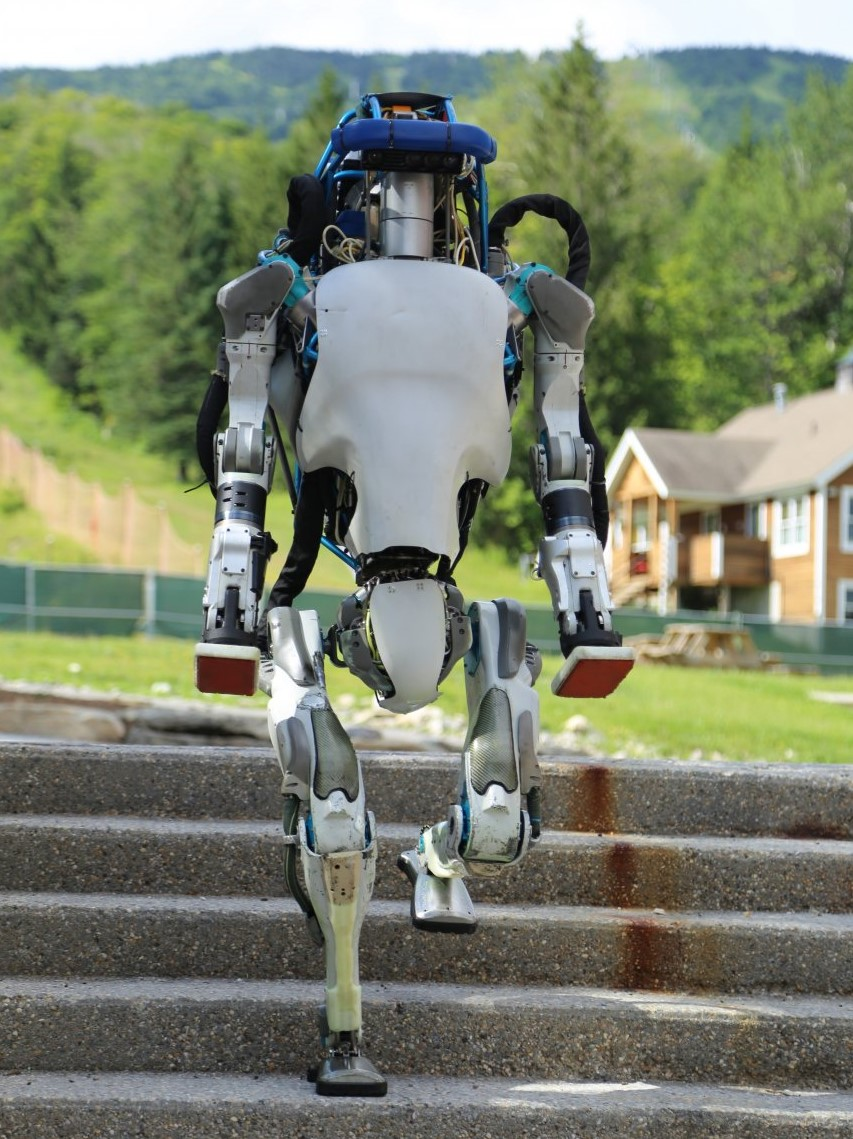
\includegraphics[width=.8\linewidth]{STYLESTUFF/AtlasNew.jpg}
   \caption{}
    \label{fig:currentrobotsa}
  \end{subfigure}
  \begin{subfigure}{0.23\textwidth}
    \centering
  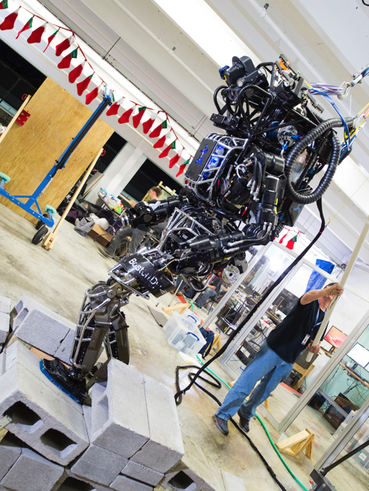
\includegraphics[width=.8\linewidth]{STYLESTUFF/AtlasOld.png}
  \caption{}
   \label{fig:currentrobotsb}
  \end{subfigure}
  \begin{subfigure}{0.23\textwidth}
    \centering
  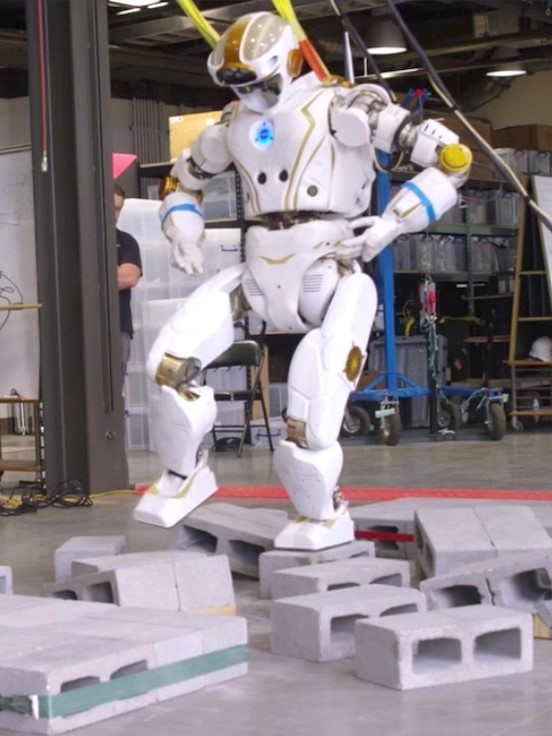
\includegraphics[width=.8\linewidth]{STYLESTUFF/Valkyrie.jpeg}
    \caption{}
     \label{fig:currentrobotsc}
  \end{subfigure}
   \begin{subfigure}{0.23\textwidth}
     \centering
  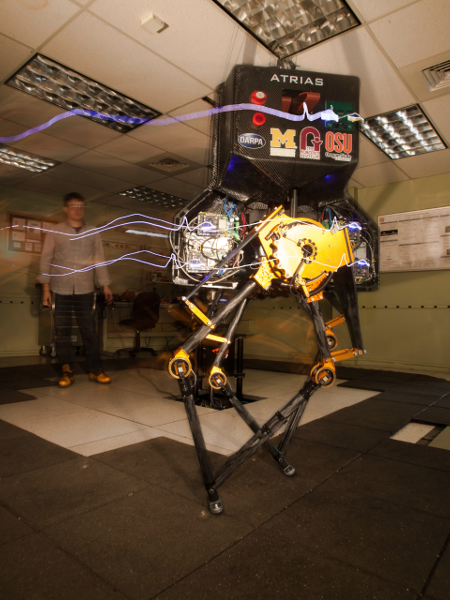
\includegraphics[width=.8\linewidth]{STYLESTUFF/ATRIAS.png}
  \caption{}
   \label{fig:currentrobotsd}
  \end{subfigure}
  \caption{A selection of currently popular humanoid robots. \textbf{(a)} Boston Dynamics' new Atlas \cite{newatlas}. \textbf{(b)} Previous version of Atlas \cite{oldatlas} and \textbf{(c)} NASA's Valkryie \cite{valkyrie} walking over rough terrain at IHMC. \textbf{(d)} ATRIAS, a bipedal robot \cite{atrias}.}
  \label{fig:currentrobots}
\end{figure}
\subsection{Modeling}
As can be seen from the images in \figref{fig:currentrobots}, a lot of bipedal robots are capable of more tasks than walking alone. As this survey is focused on walking and stabilizing by the legs, tasks as for example grasping and having environment contact of the upper body are not considered. However, even without contact the upper body plays a crucial roll in the dynamics of the robot. Chest and arm movements can create angular momentum that can control the system, which is considered in this survey. An example of the modeling of a full robot in joints and links can be found in \cite{yamaguchi1999development}.\\
\subsection{Simulation}
Because of the complexity and size of the systems considered, simulation is key. There exist multiple simulation environments, from which one of them is the open source Gazebo \cite{koenig2004design}. At IHMC an inhouse developed simulation environment is used: \ac{SCS}. This environment is written in Java.

\section{\ac{LIP} Models}
In modeling of walking, one of the most important assumptions often made is the modeling of the stance leg as a \ac{LIP}, as for example in \cite{kajita20013d}. Besides this, a not-linearized inverted pendulum is also widely used in the modeling of walking \cite{kuo2005energetic}. For planning and control however, a linearized description is desirable. In the \ac{2D} \ac{LIP} equations of motion
\begin{equation}
\ddot{x}=\frac{g}{l}x
\label{eq:LIPeom}
\end{equation}
where $l$ is the pendulum length and $x$ the Cartesian x-coordinate of the pendulum tip, the motion of the tip along the x-axis does not affect $l$. At any position $x$, a local virtual straight pendulum can be considered, so this motion is at a constant height and $l=z_0$  holds. As in \ac{3D} by the linear model the system dynamics can be decoupled, the dynamics in $y$-direction will read the same: $\ddot{y}=\frac{g}{l} y$. In \figref{fig:3dlip} this motion is visualized if the \ac{CoM} is relatively far from from the base. The pendulum base lies in the origin and $\boldsymbol{x} = [x,y]^T$ is the \ac{2D} \ac{CoM} projection on the horizontal plane. Because the \ac{LIP} assumption holds, the vertical component of the leg force $\boldsymbol{f}$ has to cancel out gravity acceleration: $f_z=mg$.
\begin{figure}[h]
\centering
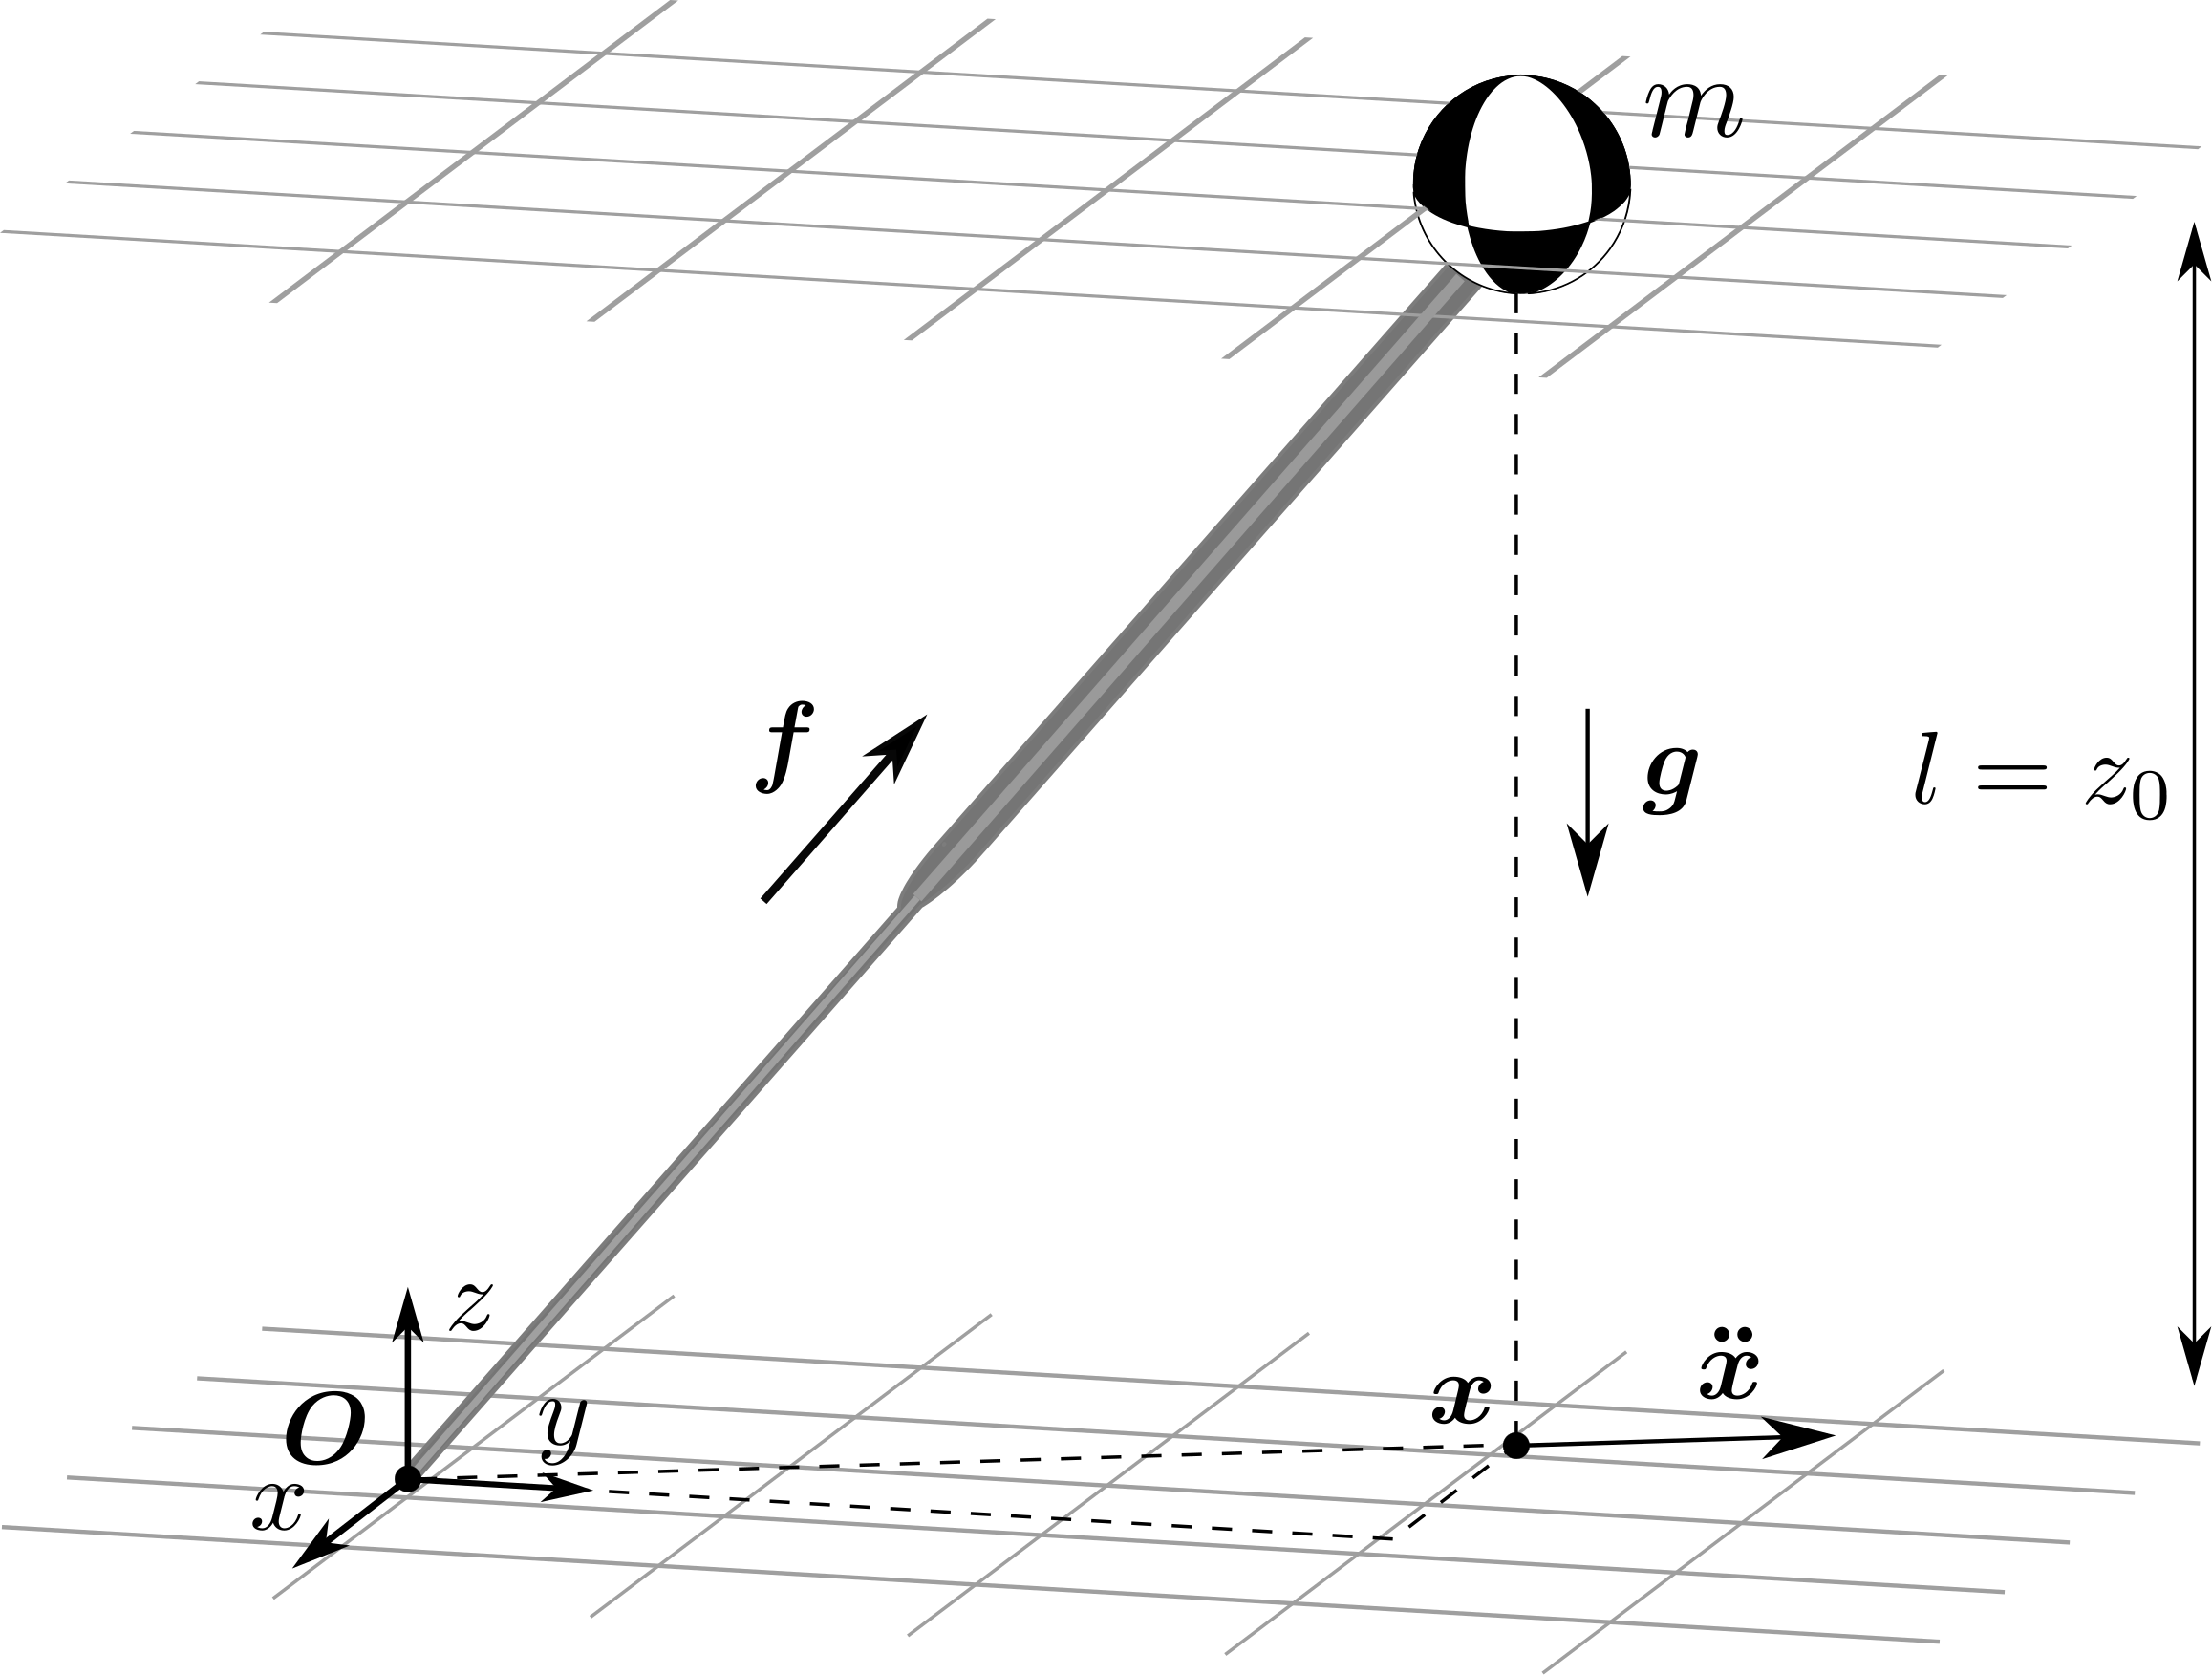
\includegraphics[width=0.5\textwidth]{STYLESTUFF/3DCoMwithoutfoot.png}
\caption{\ac{3D} motion of \ac{LIP} model.}
\label{fig:3dlip}
\end{figure}

\subsection{Conservation of \ac{Elip}}
\cite{kajita1992dynamic} had a crucial finding in an extended use of \ac{LIP} models. Because $F=ma$, $I=Fv$ and $E = Fs = \int Fv dt$, there can be reasoned that if one takes the time integral of the product of the second and the first derivative of a state, an expression for a normalized energy can be achieved: $\frac{E}{m}=\int av dt$. In the mentioned publication that same action is applied on Eq. \eqref{eq:LIPeom}:
\begin{equation}
\int (\ddot{x}-\frac{g}{l}x)\dot{x} dt = \frac{1}{2}\dot{x}^2-\frac{g}{2z_0}x +C=0
\label{eq:Elip}
\end{equation}
with $C$ the integration constant. The \ac{LIP} Orbital Energy is defined as $E_{LIP}=-C$. 

\subsection{The \acf{ICP}}
Although the finding of the \ac{LIP} Orbital Energy was very important for future robot motion modeling, more than a decade later \cite{pratt2006capture} introduced the \ac{CP}. Taking $E_{LIP}=0$ and taking the square root of Eq.  \eqref{eq:Elip} gives
\begin{equation}
x_{CP}=\sqrt{ \frac{z_0}{g}}\dot{x} 
\label{eq:cp}
\end{equation}
where $x_{CP}$ is the \ac{CP}, measured from the current pendulum tip position, based on the current tip velocity $\dot{x}$. This is the point where the velocity is driven to zero and the pendulum is upright. In \figref{fig:2dicp} a \ac{2D} visual explanation is given of this point.
\begin{figure}[h]
\centering
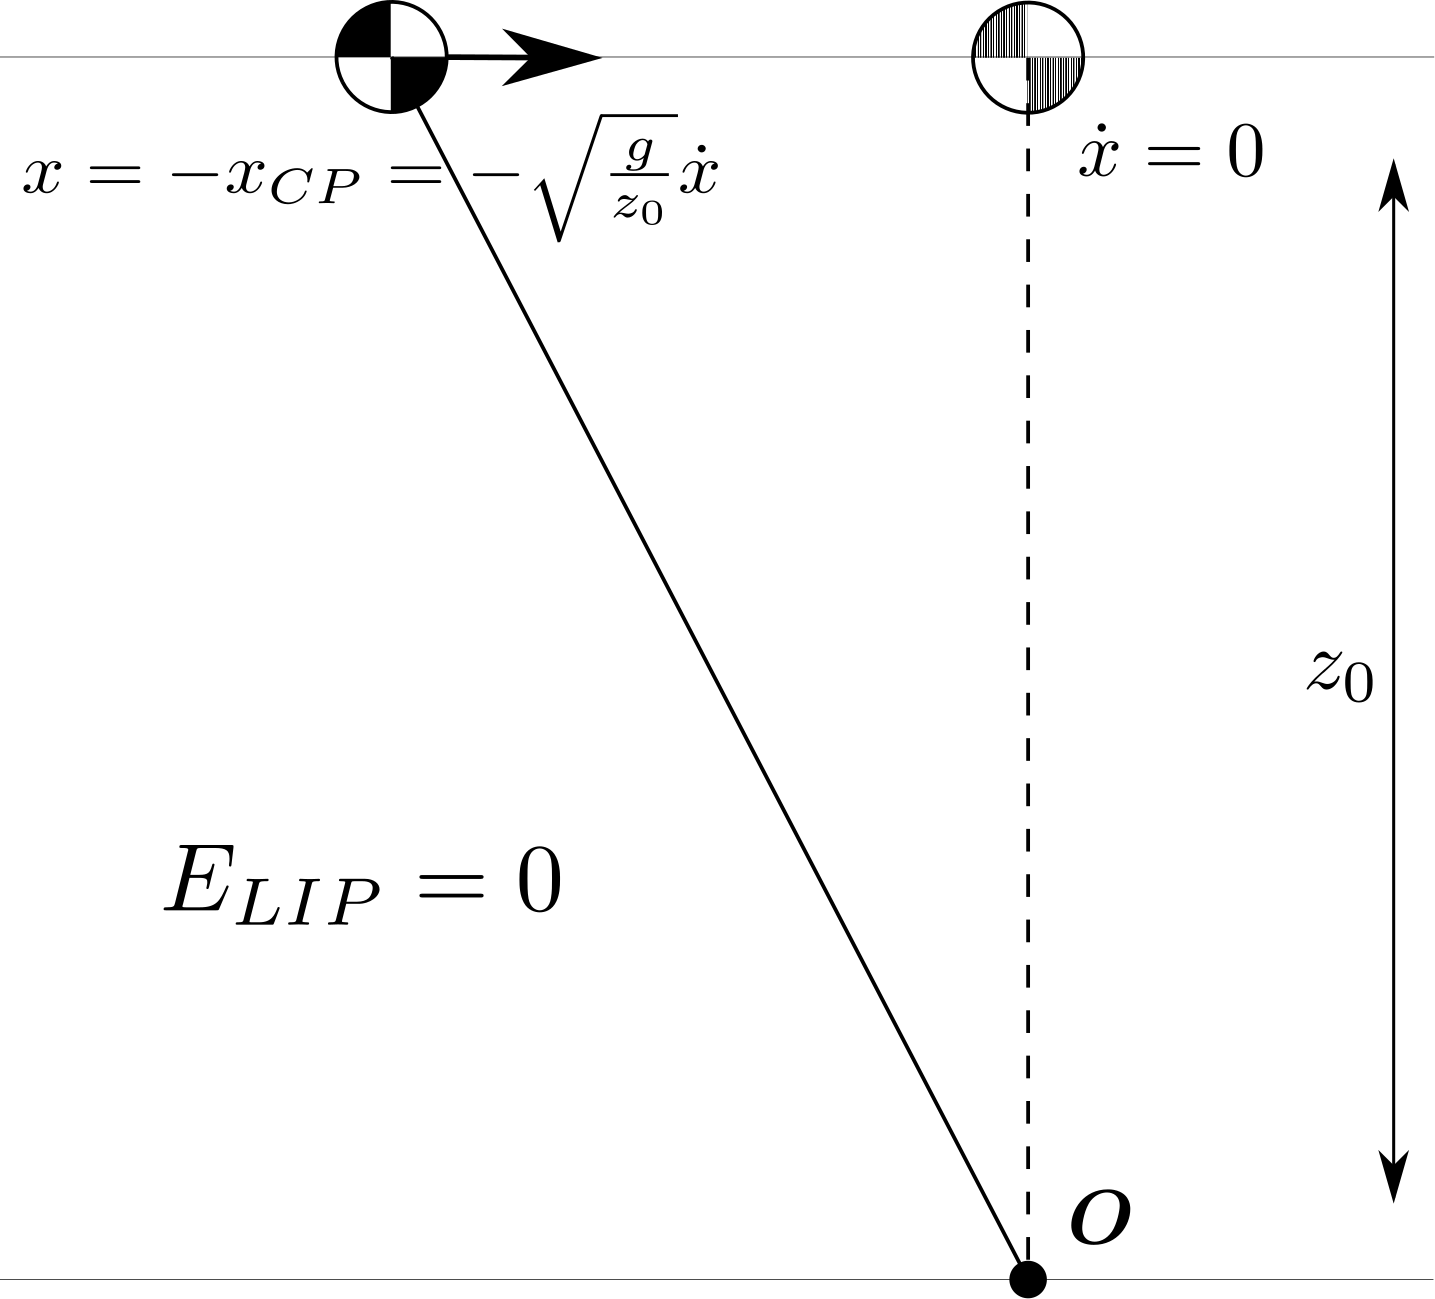
\includegraphics[width=0.4\textwidth]{STYLESTUFF/2DICP.png}
\caption{Visualization of path and states by the capture of the point mass according \ac{ICP} theory.}
\label{fig:2dicp}
\end{figure}
Later, the \ac{ICP} was introduced \cite{koolen2012capturability}, which gives a slightly different discription of the point:
\begin{equation}
x_{ICP}=x+\sqrt{ \frac{z_0}{g}}\dot{x} 
\label{eq:icp}
\end{equation}
where $x_{ICP}$ is the \ac{ICP}. In this way, the point can be described in the environment coordinates.
The $x$- and $y$ coordinate can be decoupled as in the equation of motion of Eq. \eqref{eq:LIPeom}. However, in the \ac{2D} horizontal plane it is not guaranteed that the velocity direction of the \ac{CoM} is towards the ankle point. 
\subsubsection{\ac{ICP} dynamics}
Because the ankle is not always located at the same location as the \ac{ICP} for the current horizontal velocity, for modeling and planning the time derivative is taken of the \ac{ICP}, which is named the \ac{ICP} dynamics \cite{koolen2012capturability}. This time derivative can be written as a function of the current \ac{ICP} location:
\begin{equation}
\boldsymbol{\dot{x}}_{ICP}=\sqrt{ \frac{g}{z_0}}\boldsymbol{x}_{ICP} 
\label{eq:cp}
\end{equation}
where $\boldsymbol{x}_{ICP}$ is the $xy$-vector of the \ac{ICP} location and assuming that the pendulum base is the origin.

\section{Humanoid Robot Terminology}
As the \ac{ICP} is a measure for the behavior of a bipedal robot, there exist plenty of terms and descriptions for specific virtual points and forces on and acting on the robot. In this section a short summary is given from the most popular jargon.

\subsection{The \ac{CoP}}
The larger feet of a human than those of a dog make him more capable of upright walking, due to an increase of controllability of the modeled-as-\ac{LIP} human. The ankles can apply a torque that would virtually move the position of the base of the inverted pendulum, so that the linear acceleration on the \ac{CoM} as in Eq. \eqref{eq:LIPeom} and the capture point as in Eq. \eqref{eq:cp} change. The new virtual base is called the \ac{CoP}. By its definition, this point only lives within the foot polygon \cite{vukobratovic2004zero}. In \figref{fig:3dlipfoot} the definition of the \ac{CoP} is visualized. If the point mass is restricted to move on a constant height, the vertical component of $\boldsymbol{f'}$ counteracts gravity: $f'_z=g$. 
\begin{figure}[h]
\centering
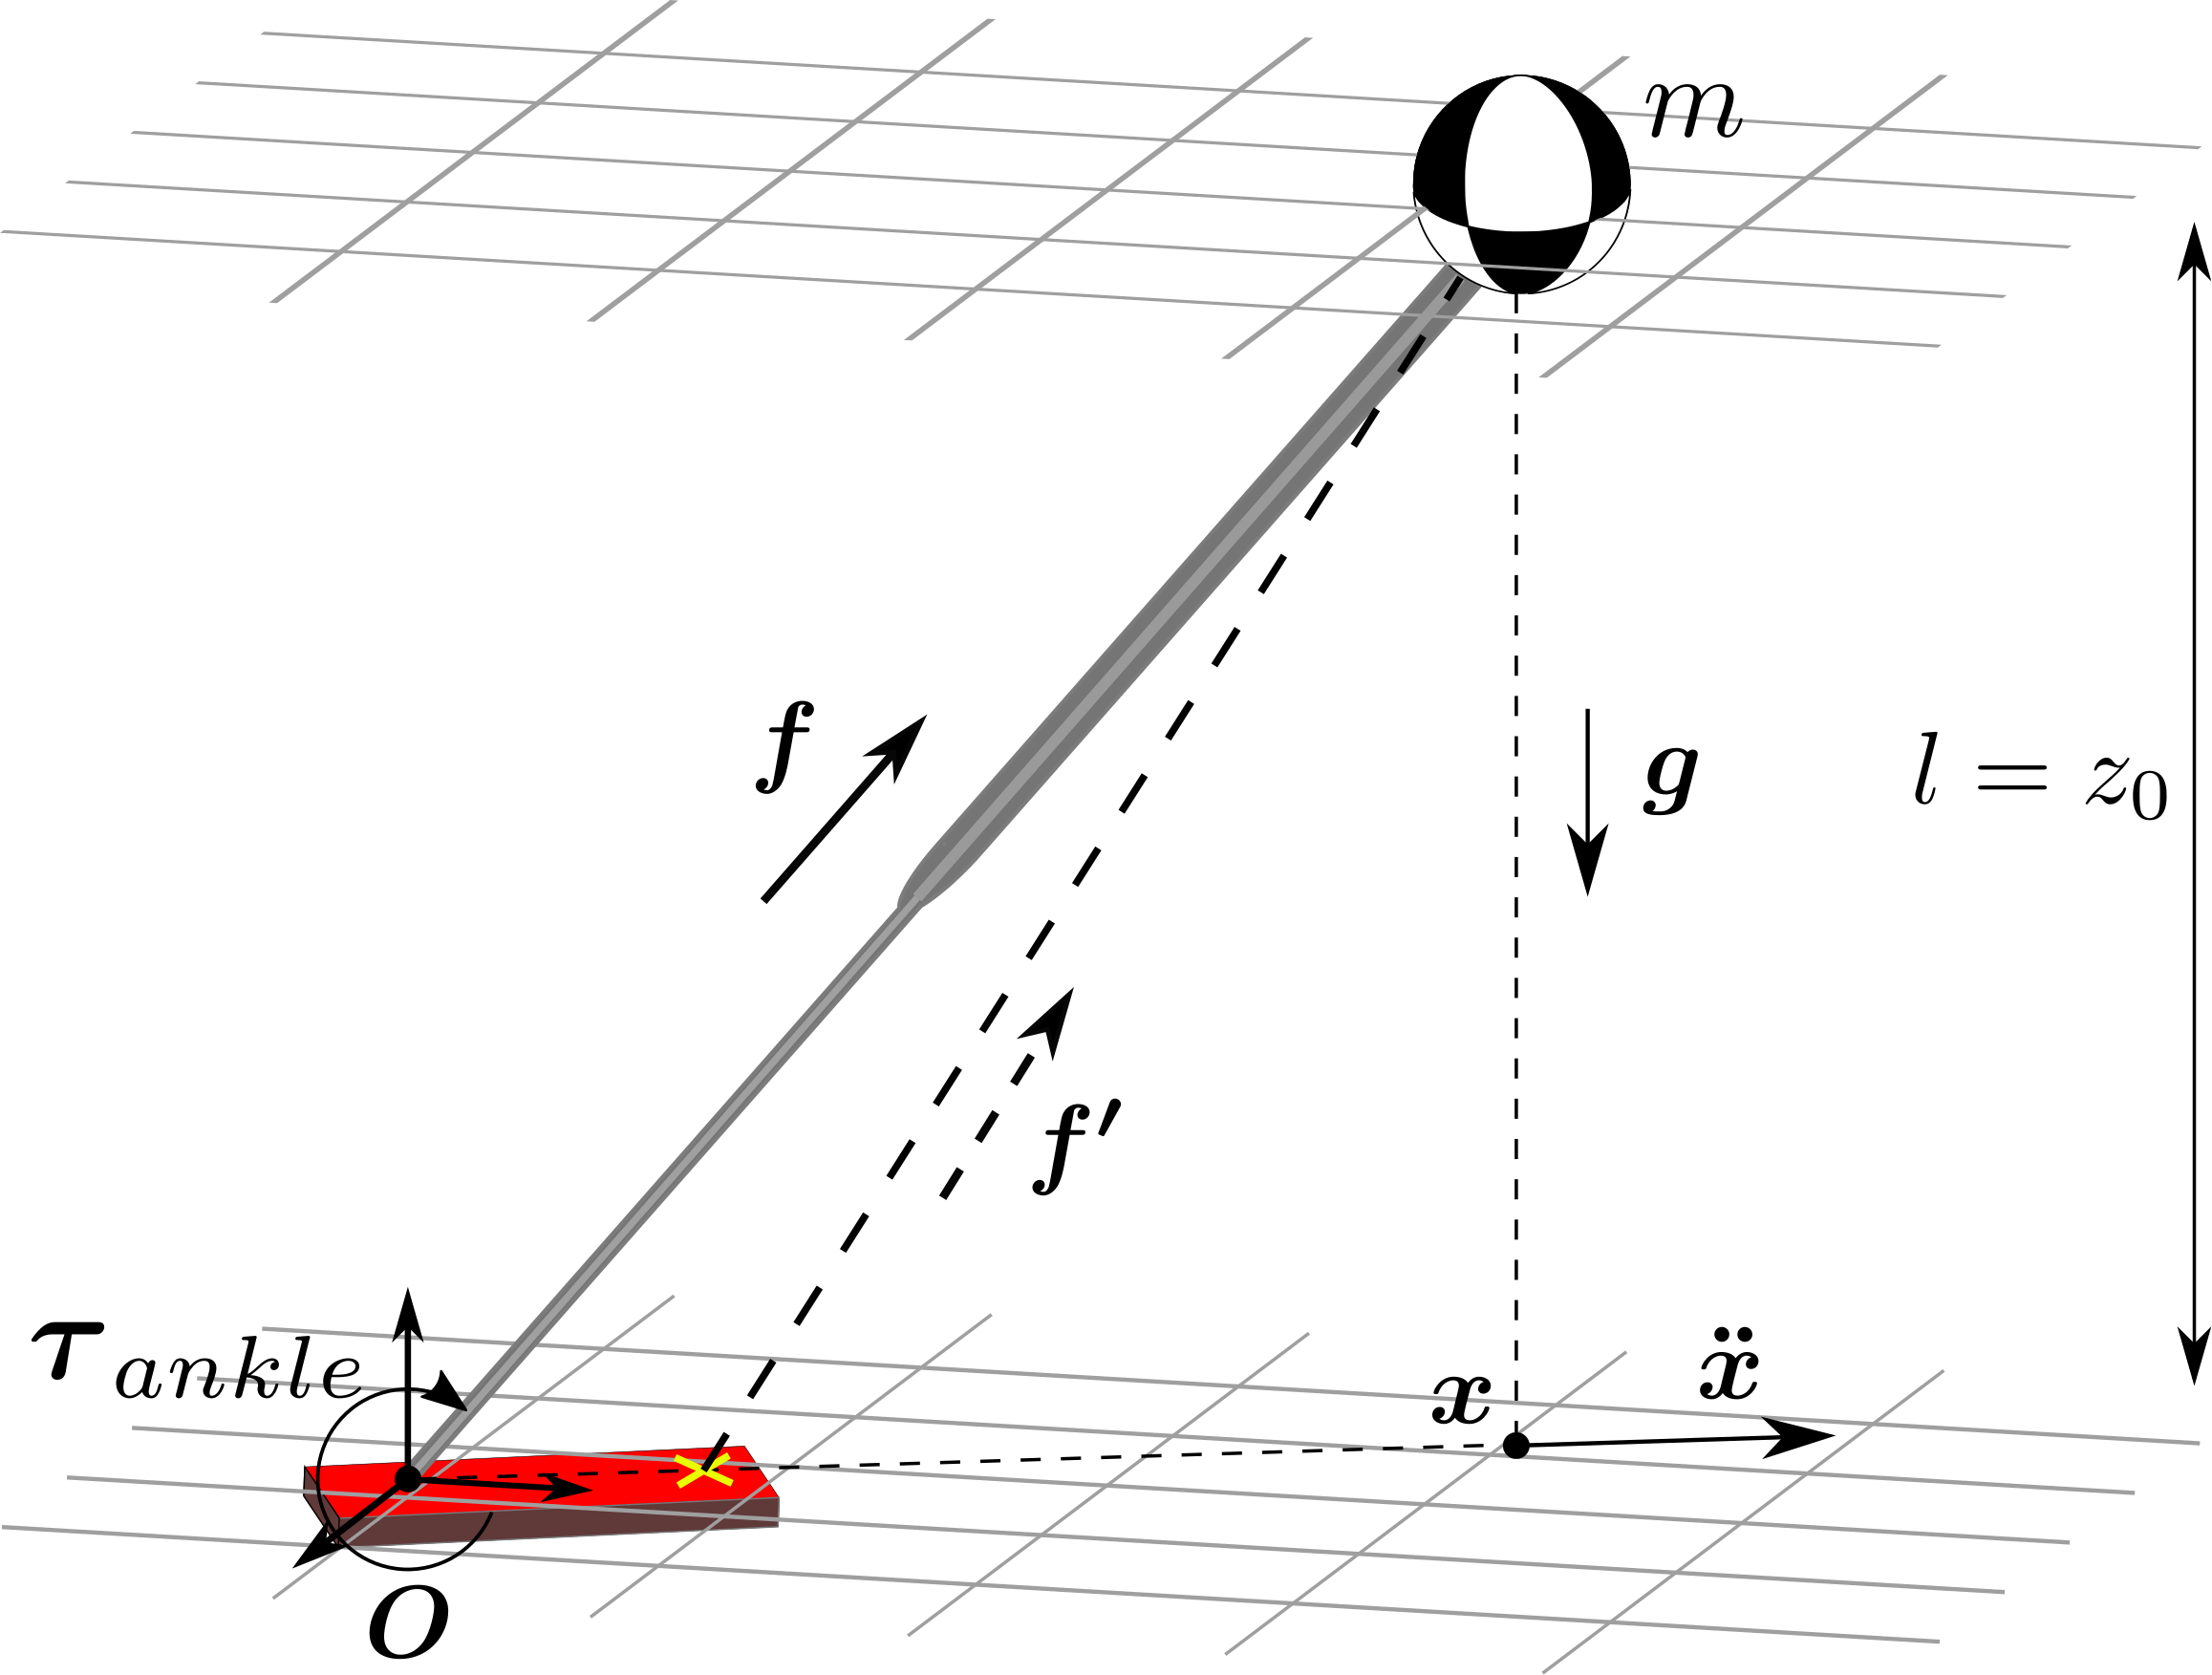
\includegraphics[width=0.5\textwidth]{STYLESTUFF/3DCoMwithfoot.png}
\caption{\ac{3D} motion of \ac{LIP} model with foot. The yellow cross points out the \ac{CoP} location.}
\label{fig:3dlipfoot}
\end{figure}

\subsection{The \ac{ZMP}}
The \ac{ZMP} coincides during stable walking with the \ac{CoP}, like described in \cite{vukobratovic2004zero}. The two points however are not equal in unstable or more complicated cases, like falling over.  The \ac{CoP} is restricted to be in the foot polygon, as this is a point that links to contact forces \cite{sardain2004forces}. The \ac{ZMP} however is not restricted to lie within the foot polygon. The \ac{ZMP} is the point on the ground where the tipping moment equals zero. The tipping moment is defined as the component of the moment that is tangential to the ground surface. The \ac{ZMP} initially was introduced in \cite{vukobratovic1969contribution}.

\subsection{The \ac{CMP}}
The earlier mentioned points give sufficient measure for a \ac{LIP} model with point mass and finite sized feet. However, any angular momentum applied by the body does not affect those points. In the case of the \ac{CoP} for example, the model assumes the resulting reacting force acts from the \ac{CoP} through the \ac{CoM} The \ac{CMP} takes angular momentum into account, which can be used as a measure and for control \cite{popovic2005ground}. This is defined as the point where a line passing through the \ac{CoM}, parallel to the ground reaction force intersects with the ground surface. The \ac{CMP} is defined as
\begin{eqnarray}
x_{CMP} = x_{ZMP} + \frac{\tau_{y,CoM}}{F_{gr,z}}\\
y_{CMP} = y_{ZMP} - \frac{\tau_{x,CoM}}{F_{gr,z}}
\end{eqnarray}
where $\tau_{CoM}$ is the torque around the \ac{CoM}, $[x_{ZMP},y_{ZMP}]$ the \ac{ZMP} location on the horizontal plane and $F_{gr,z}$ is the ground reaction force in z-direction in Cartesian space. In \figref{fig:3dlipfootinertia} it is displayed how the body angular momentum affects the ground reaction force $\boldsymbol{f'}$ from the \ac{CoP} and how the \ac{CMP} can be determined with the intersection of a parallel line through the \ac{CoM} and the ground plane. For clarity the point in the image lies on the line from $\boldsymbol{O}$ to $\boldsymbol{x}$. This has not to be the case however, as the body can exert angular momentum along all axes. 
\begin{figure}[h]
\centering
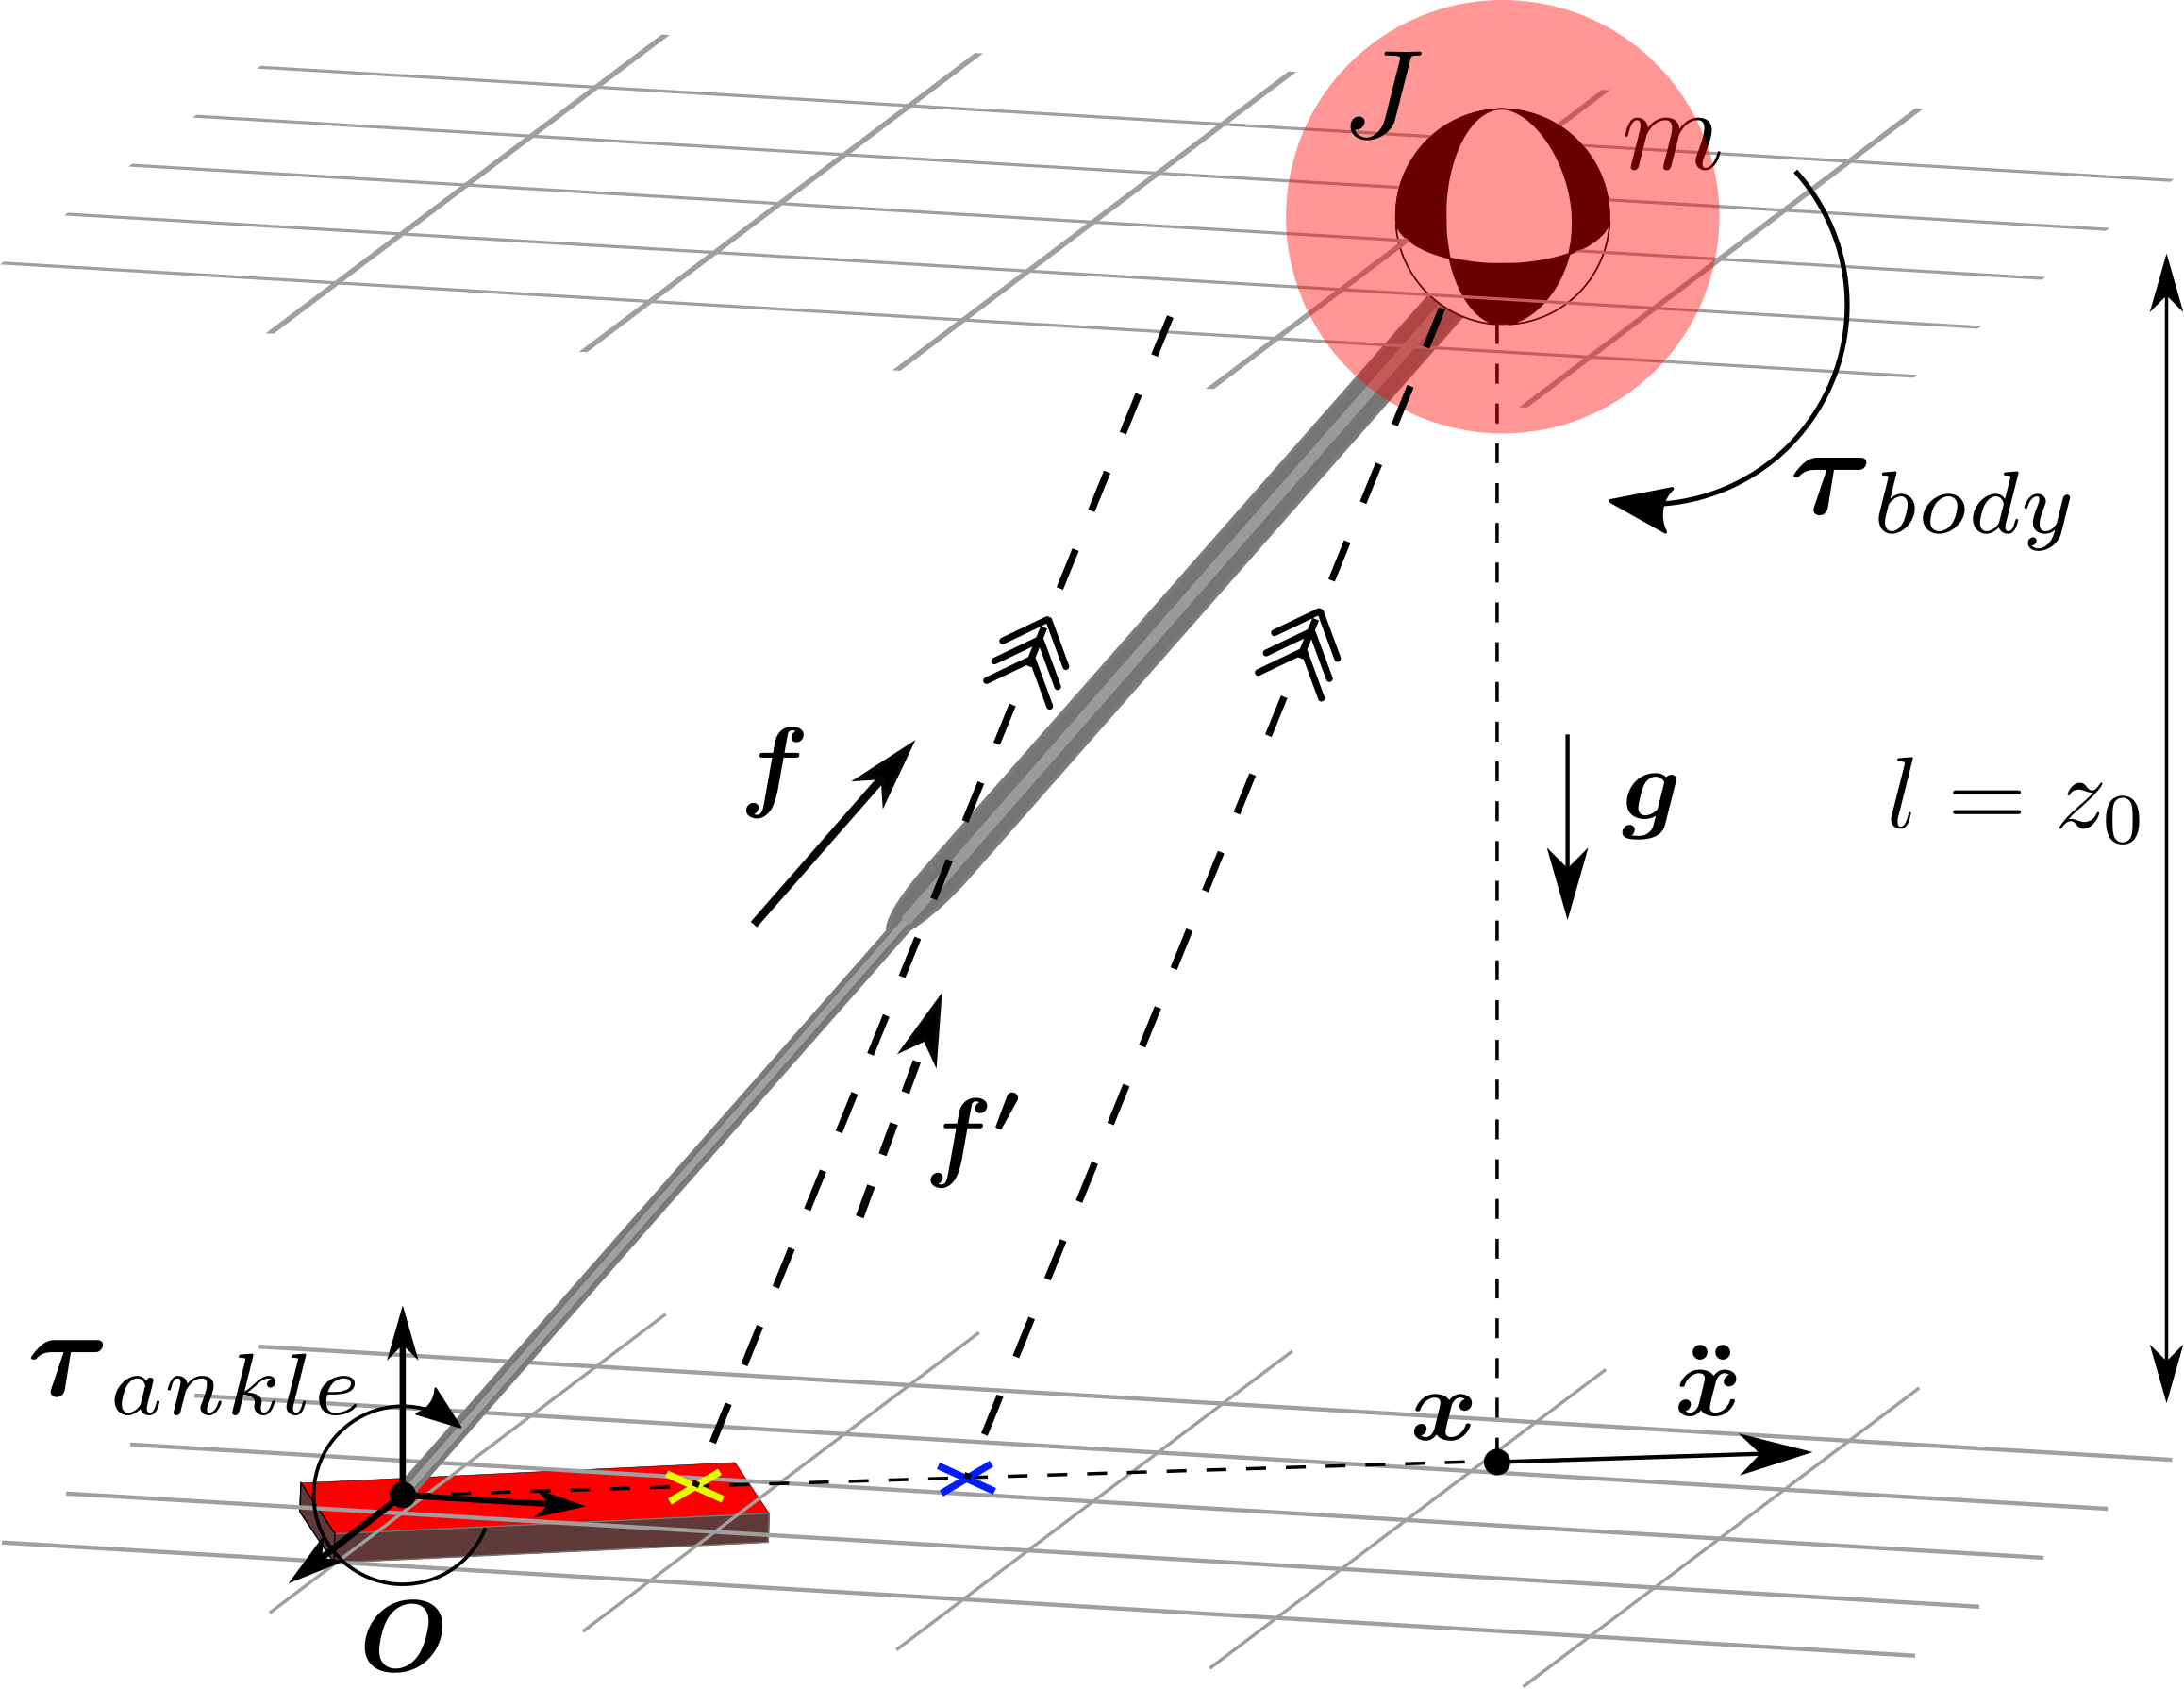
\includegraphics[width=0.5\textwidth]{STYLESTUFF/3DCoMwithfootinertia.png}
\caption{\ac{3D} motion of \ac{LIP} model with foot and body inertia. The blue cross points out the \ac{CMP} location.}
\label{fig:3dlipfootinertia}
\end{figure}
\subsection{Linear momentum rate}
To combine the effects described in this section in one single measure, often the linear momentum or linear momentum rate is considered in the horizontal plane. This boils down to be a combination of the \ac{LIP} equations of motion and the \ac{CoP}, \ac{ZMP} or \ac{CMP}. Using the \ac{CMP} the linear momentum rate is then defined as
\begin{equation}
\boldsymbol{\dot{l}} = m\boldsymbol{\ddot{x}}= m\frac{g}{z}(\boldsymbol{x}-\boldsymbol{x}_{CMP})
\label{eq:ldot}
\end{equation}
where $\boldsymbol{\dot{l}}$ is the linear momentum rate in the horizontal plane, $\boldsymbol{x}$ the \ac{2D} \ac{CoM} position and $\boldsymbol{x}_{CMP}$ the \ac{CMP} position.
\subsection{Other points}
Other than the points mentioned before, there are sometimes other points considered in humanoid robotics. Examples of this are the \ac{eCMP} and the \ac{VRP} \cite{englsberger2013three}, but those are not further discussed here. 

\section{Analysis \& Discussion}
From the study in this chapter it becomes clear that oftentimes the complex system of a walking robot is captured in a relatively simple model, namely that of a \ac{LIP} with a mass with inertia on the tip and a base that is maneuverable within limits. The combined dynamics of this configuration define the dynamics in the horizontal plane of the \ac{LIP}. This however requires the nominal ground reaction force to have a vertical component equal to the force applied by gravity. For motion over a flat surface, it seems intuitively as a desirable goal to have a constant height. If the goal is to move somewhere in the planar world, height variation and thus height acceleration would only waste energy. However, for having a walking motion where the gravity vector is not perpendicular to it, the assumption of the constant force in vertical direction might not be a solid assumption. Even on a flat surface the \ac{CoM} varies slightly in height \cite{lee1998determinants}. Moreover, varying leg force could be used to accelerate or stop quicker, which would mean a different force is applied than assumed in the \ac{LIP} model. The different leg force changes the horizontal component of the force, which can control the motion. This also results in a change of its vertical component, which after time changes the \ac{CoM} height, as it is not equal to gravitational forces anymore.
%
\chapter{Planning, Control \& State Estimation}%
\label{chap:planningcontrol}
In this chapter the most common planning, control and state estimation strategies are pointed out and reviewed. As mentioned before, publications that regard the humanoid robots in use at IHMC, get special consideration.

\section{Planning}
In robotics, the planning problem can be described with a desired final goal of the motion, constraints on the path itself as terrain where collision needs to be avoided and constraints on the capabilities of the system as kinematic limits and actuation limits. As the dynamics of a humanoid robot are complex and underactuated, there exist numerous way to generate a walking plan. This typically ranges from reactive stepping and tracking a desired velocity to precise foot placements. In this section common planning strategies are described.

\subsection{Footstep planning}
While not all bipedal robots require a footstep plan to walk, most humanoids do. A footstep plan is a sequence of foothold references on the ground. Those can be computed either offline or online. Offline, either an autonomous planner can make a plan, or a robot operator can define desired footsteps manually. Online the robot in some cases can re-plan to avoid collision or adjust a footstep to use for stabilization. In \cite{chestnutt2005footstep} is described how an online plan can be generated as an example. At IHMC, based on LiDAR terrain information from the robot's head, the operator can define footholds which in the \ac{GUI} turn green or red for kinematic reachability. There is also worked on algorithms to adjust steps real-time for stability \cite{griffin2017walking} and autonomous planners based on for example the A\textsuperscript{*} algorithm. As footstep planning can be decoupled from the varying height problem, the footstep plan is assumed to be given beforehand in this survey.

\subsection{Dynamic planning}
Through the history of humanoid robots, there are various strategies used to generate a body path plan. There are differences in planning in joint-space and planning only a \ac{CoM}, \ac{CoP} or \ac{ICP} trajectory for example. This is greatly depending on the control strategy that is used, but also on the complexity of the robot. Currently at IHMC an \ac{ICP} plan is generated based on a footstep plan with \ac{CoP} knot points \cite{englsberger2014trajectory}. Based on the desired time of the footstep plan, the \ac{ICP} dynamics are integrated backwards in time to come to a reference trajectory. This plan is tracked using PD-control, where the \ac{CMP} is used as control input to achieve the desired \ac{ICP} plan. During the double support phase the \ac{LIP} assumption is not valid, and the \ac{ICP} trajectory is here moved between two footsteps by a time polynomial.  

\subsection{Swing leg trajectories}
If the robot places its foot from the current footstep to the next, a more local plan is generated. This is often done by defining a polynomial spline from the one foothold to the other, with knot points at a certain height above the ground to make the foot not hit the ground. This spline can be generated as a set of piece-wise minimum jerk trajectories. The minimum jerk trajectory minimizes the jerk, the third derivative of position with respect to time, and needs a desired completion time for the trajectory as input. This desired time for the entire spline is called the desired swing time for this step. In \figref{fig:scsval} swing leg trajectories are displayed in the simulation environment of \ac{SCS}, together with among other things a footstep plan.

\begin{figure}[h]
\centering
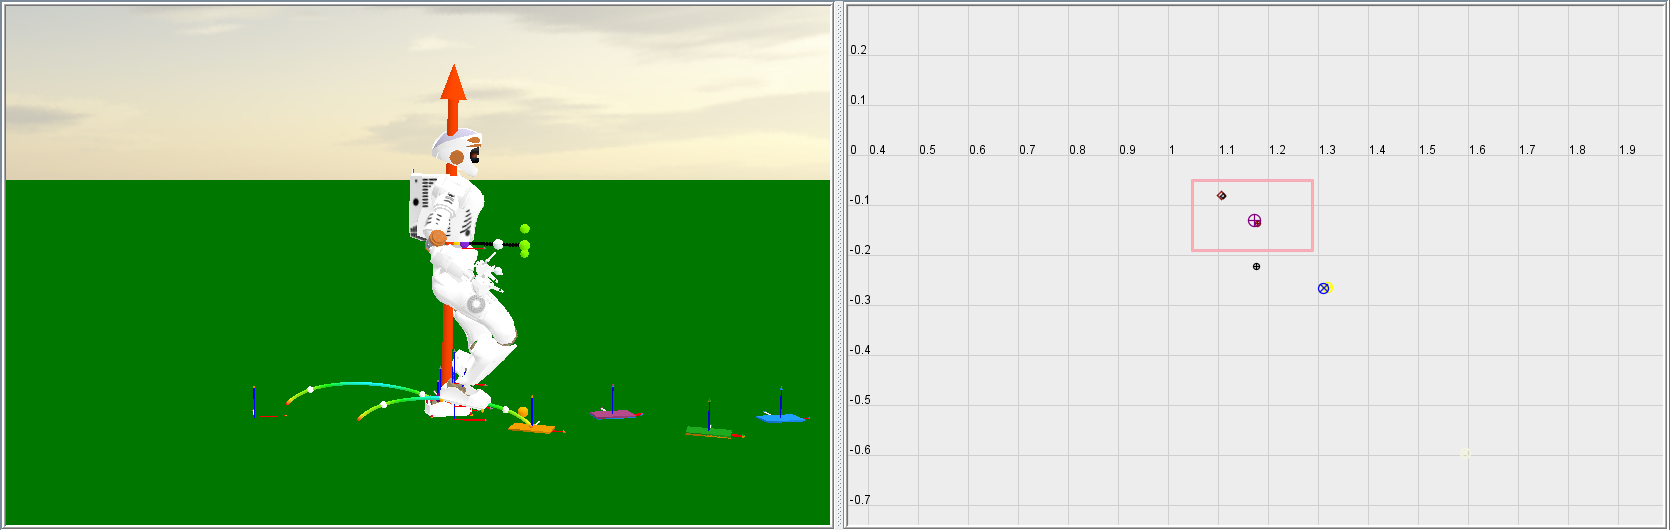
\includegraphics[width=0.8\textwidth]{STYLESTUFF/SCSValSS.png}
\caption{Valkyrie walking in \ac{SCS}. In the left window a footstep plan is made visible together with the swing leg trajectories with their knot points. The red arrow indicates the ground reaction wrench and the window on the right displays the current ground contact with some reference and measured points.}
\label{fig:scsval}
\end{figure}

\section{Control}
To track a generated high level plan the system has to be controlled. PID-control, LQR and MPC are all used in humanoid robotics. Again, there are differences in joint-level control and for example the control of the desired \ac{CoM} position, which often are separated in high level and low level control. In some cases, like with the \ac{HZD} approach as described in \cite{westervelt2003hybrid}, there is no decoupling between such levels. However, the \ac{HZD} is for this reason often applied to simpler robots, as in the mentioned paper and on ATRIAS. Furthermore, the \ac{HZD} approach is designed for systems with a degree of underactuation of one, which corresponds more to a \ac{2D} than a \ac{3D} robot model. 
\subsection{High level control}
Tracking the \ac{ICP} trajectory as is done at IHMC is an example of high level control. The robot in this stage can be seen as a \ac{LIP} with a finite sized foot and body angular momentum. At a current footstep, using the right combination of ankle torque and angular momentum, the robots motion can in theory be controlled considering the simplified \ac{LIP} model. The robot is assumed to keep itself at a constant height and expected to generate the desired centroidal momentum. Simplification of the model to only a \ac{CoM}, angular momentum and a ground reaction force, makes control more accessible than looking at joint level. The desired values of the high level controller are send to a mid level controller to translate this information to joint level control.
\subsection{Mid and low level control}
As the real robot is not a \ac{LIP} and cannot generate high level control inputs as angular momentum as a single control input, other layers of control are needed: mid and low level control. Low level controllers are often based on inverse kinematics and inverse dynamics. This concept is also widely used in industrial robotic manipulators, as for example in \cite{asada1990inverse}. What often the basis is for desired motions on joint scale is the fact that so called centroidal dynamics about the pelvis or \ac{CoM} have to equal the wrenches applied on the environment, as for example in \cite{kajita2003resolved} and \cite{koolen2016design}. An important constraint on wrenches applicable on the environment is the unilaterality of the contact and the available contact friction. This is often captured in having a so called wrench cone above the foot, wherein the resulting ground wrench has to lie. The centroidal dynamics are a combination of the linear and angular momentum rate. In \figref{fig:controlframework} an overview of the controller structure at IHMC is given. The momentum rate of change objective consist during walking mainly of the linear momentum rate as in Eq. \eqref{eq:ldot}. The motion tasks are for example moving the swing leg. This information from the high level controller is then translated in a quadratic program, that defines the solution as a set of joint accelerations and reaction wrenches. This is translated to joint level with inverse dynamics.
\begin{figure}[h]
\centering
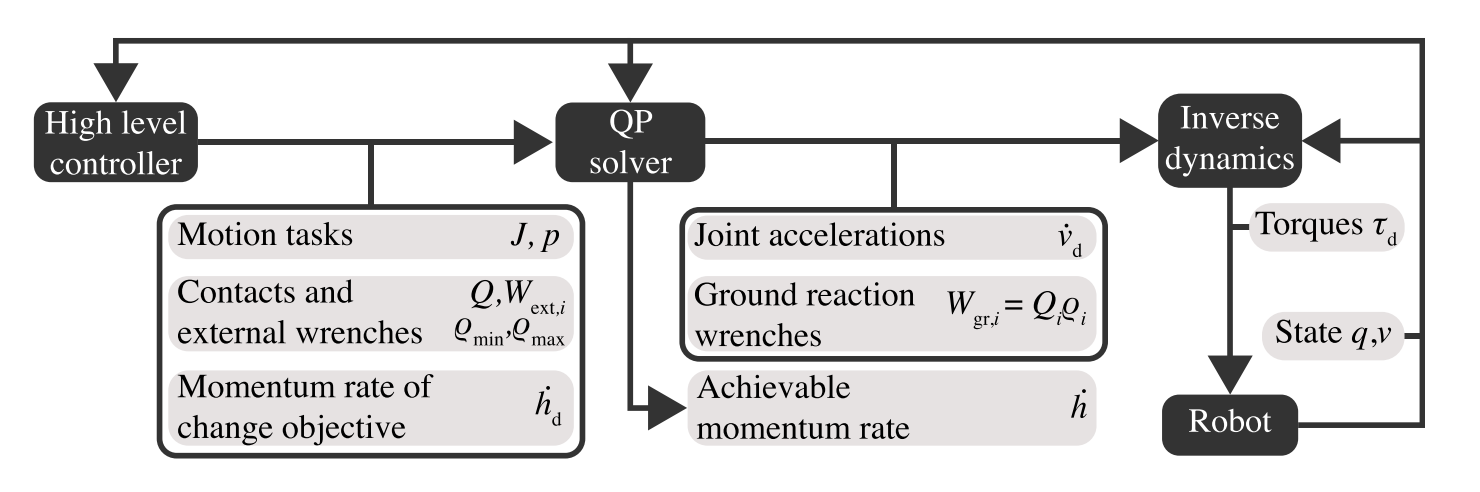
\includegraphics[width=0.8\textwidth]{STYLESTUFF/controlframework.png}
\caption{Overview of control framework used at IHMC, retrieved from \cite{koolen2016design}}
\label{fig:controlframework}
\end{figure}
\subsection{Compliant control}
In the walking of a bipedal robot with legs hybrid switching between swing and stance, a problem gets introduced with this hybrid phase shift. During swing, a trajectory is tracked using a control strategy that links more to position tracking. When the foot hits the ground, it switches instantly to the stance phase, where its position is fixed and its control actions are mainly based on forces. This instant switch can cause instabilities in the controller and an agile, compliant control strategy is needed. In \cite{sentis2006whole} is described how for different phases a different set of controller gains can be used to deal with the difference of impedance needed in control. 

\section{State Estimation} 
As state estimation is dependent on the available sensor data and the quality of the data, the possible strategies for estimation depend on the particular robot model. Typically, the robot has position sensing in all joints, that sometimes have torque sensing as well. An \ac{IMU} can be present in the body, or even in some body parts. State estimation of for example the pelvis orientation and velocity can be done by combining sensor data from both the body \ac{IMU} and an inverse dynamics algorithm that uses information from joints. On joint level, a low-pass filter can be applied and then based on the dynamics of the robot, a heuristic approach in combining the \ac{IMU} and joint data can be used to estimate the pelvis state, as is done in \cite{koolen2016design}. Another possibility is the use of more sophisticated sensor fusing techniques as the \ac{EKF}, as in \cite{kuindersma2016optimization}. Due to the complexity of the system this can be however challenging, especially with application on hardware. 

\section{Analysis \& Discussion}
The entire framework to plan and control the motion of a humanoid robot is so extensive, that it is important to narrow the areas of focus. The knowledge gained from the investigation for this chapter gives a good basis of understanding what the current bottle necks in humanoid robot control and planning are. The current frameworks do not regard any height variation of the inverted pendulum model most of the times, which of course is not done without reasons. First, a linearized model is very desirable in control, as the computational cost of such is much lower than with nonlinear ones. Second, with the linear model a plan through the \ac{3D} world can by dynamics mostly captured in a \ac{2D} plan, which simplifies the planning problem a lot. \\
For a varying height model the computation time might be an important aspect, especially for control and online planning, as full pendulum or robot dynamics are nonlinear. This has to be taken into consideration. 
%
\chapter{Varying CoM Height}%
\label{chap:varyingheight}
As mentioned earlier, recently work has been done in removing the constant height assumption from the walking model. The motivation for this is threefold. The use of height can be used in tracking control. Where angular momentum and the \ac{CoP} are often the two control inputs for a \ac{LIP} model of the current swing phase, the use of height, thus a varying leg force, can be used as a third input. Furthermore, in motion over un-flat terrain a varying height model can give a better approximation of how the dynamics will behave over time. Even over flat terrain, the \ac{CoM} trajectory of a human does not follow a straight line, where the dynamic behavior differs from the \ac{LIP} assumption. In other words: both control and planning can be improved. \\
Before there is looked at different approaches, a system description for a \ac{2D} inverted pendulum with a point mass on the tip with varying length is defined. Because the force the pendulum applies on the point mass does not have to be equal to the gravitational acceleration in its vertical component, the system can be described as a traveling point mass subject to a force coming from a point on the ground. This is visualized in Figure \ref{fig:2dnonlin}.
\begin{figure}[h]
\centering
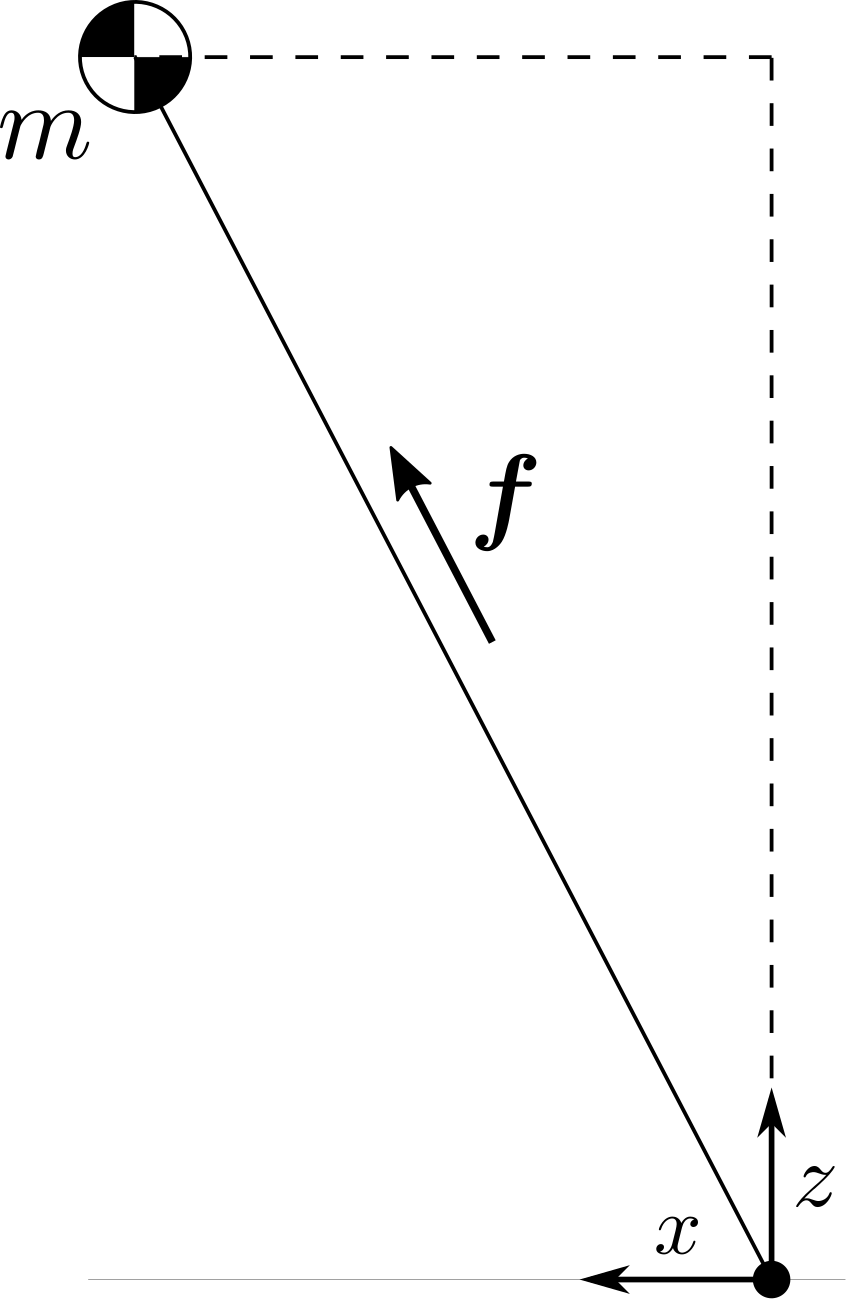
\includegraphics[width=0.25\textwidth]{STYLESTUFF/2Dnonlin.png}
\caption{Nonlinear simplified system in \ac{2D}.}
\label{fig:2dnonlin}
\end{figure} 

The non-linear model of a traveling \ac{CoM} subject to a force coming from the $[0,0]$ point on the ground is for the \ac{2D} $xz$-plane
\begin{eqnarray}
m\ddot{x} = F \frac{x}{\sqrt{x^2+z^2}}\\
m\ddot{z} = -mg+F \frac{z}{\sqrt{x^2+z^2}}
\label{eq:nonlindyn}
\end{eqnarray} 
where $F=||\boldsymbol{f}||$ is the leg or ground reaction force and $[x,z]$ the position of the point mass.


\section{Orbital Energy for Nonlinear \ac{CoM} Trajectories}
The nonlinear equations of motion of Eq. \eqref{eq:nonlindyn} are used in \cite{pratt2007derivation}. The authors constrain $z=f(x)$ and integrate the equations of motion over time, how a similar conservation of orbital energy as in Eq. \eqref{eq:Elip} is derived. This orbital energy however is not required to be a straight line trajectory, but depends on the function $f(x)$. The  full integration can be found in the paper, but the final expression writes as
\begin{equation}
   E_{orbit} = \frac{1}{2}\dot{x}^2\bar{f}^2(x)+gx^2f(x) - 3g\int_{x_0}^xf(\xi)\xi d\xi = \frac{1}{2}\dot{x}_0^2\bar{f}^2(x_0)+gx_0^2f(x_0).
\end{equation}
where $\bar{f}(x)=f(x)-f'(x)x$, $[x_0,\dot{x}_0]$ is the initial horizontal state and velocity and $[x,\dot{x}]$ is the current horizontal state and velocity. There is experimented in simulation with a symmetric polynomial, where the trajectory is tracked using a PD feedback scheme where the leg force is the control input. The polynomial description makes the integral directly solvable, based on the initial and current state. To make a clear separation between \ac{Elip}, this energy form will be defined in this report as \ac{Eorbit}.\\
Recently, this is used in a \ac{MPC} formulation and basic simulations have been done in \cite{koolen2016balance}. The main idea in this paper is to define four constraints on the trajectory $f(x)$, which define the four constants of a cubic polynomial by a matrix inversion. Those consist of two constraints on the initial conditions, one constraint on the final condition and one constraint on the conservation of \ac{Eorbit}. The matrix inversion is done offline, so that the control input can directly be written as a function of the polynomial constants and thus as a function of the initial and final states. 

\section{\ac{DCM} for Varying Height}
A couple of attempts in the use of varying height are found in adaptations of the \ac{ICP}. A couple of variations on the \acf{DCM} are examples of this. There exist multiple definitions of this \ac{DCM} and for clarity different mentions are explained and compared, as some of them seem to be interesting with respect to height usage. For simplicity and comparability, in all coming equations the mentions of \ac{CoP} and \ac{ZMP} in the publications are set to zero. In \cite{takenaka2009real} the \ac{DCM} is defined as 
\begin{equation}
q = x + \frac{1}{\omega_0}\dot{x}
\label{eq:takenakadcm}
\end{equation} 
based on a \ac{LIP} model, where $[x,\dot{x}]$ is the \ac{CoM} position and velocity and $q$ is the \ac{DCM}. Thus, this point is the same as the \ac{ICP} from Eq. \eqref{eq:cp} plus the \ac{CoM} horizontal location. \\
In \cite{englsberger2013three} the \ac{DCM} is defined as a \ac{3D} point. This is used in a un-even terrain path planner. The \ac{DCM} is here defined as
\begin{equation}
\boldsymbol{\xi} = \boldsymbol{x} + b\boldsymbol{\dot{x}}
\label{eq:englsdcm}
\end{equation}
where $\boldsymbol{\xi}=[\xi_x,\xi_y,\xi_z]^T$ is the \ac{DCM}, $\boldsymbol{x}=[x_{CoM}, y_{CoM}, z_{CoM}]^T$ and $\boldsymbol{\dot{x}}=[\dot{x}_{CoM}, \dot{y}_{CoM}, \dot{z}_{CoM}]^T$ are the \ac{CoM} position and velocity and $b>0$ is the time-constant of the \ac{DCM} dynamics. \\
\cite{hopkins2014humanoid} uses this and defines the constant $b=1/\omega_0$, where $\omega_0=\sqrt{\frac{g}{z_{CoM}}}$. This makes it again the same as the \ac{ICP}, but with a $z$ component in the state. The \ac{DCM} is derived with respect to time, where $\omega$ is posed to be time varying, so the height is time varying. This brings a new expression and is called the time varying \ac{DCM}, where the derivative is written as
\begin{equation}
\boldsymbol{\dot{\xi}}=(1-\frac{\dot{\omega}}{\omega^2})\boldsymbol{\dot{x}}+\frac{1}{\omega}\boldsymbol{\ddot{x}}
\end{equation}
where $\omega$ is the so called time varying natural frequency of the inverted pendulum.\\
\cite{caron2018capturability} mentions it uses the \ac{DCM} from Takenaka et al. and writes this as 
\begin{equation}
\boldsymbol{\xi}(t) = \boldsymbol{\dot{c}}(t) + \omega(t)\boldsymbol{c}(t)
\label{eq:carondcm}
\end{equation}
if the \ac{CoP} vectors are set to zero, where $[\boldsymbol{c},\boldsymbol{\dot{c}}]$ is the \ac{3D} \ac{CoM} position and velocity and $\boldsymbol{\xi}$ is the \ac{3D} \ac{DCM}. This is used in a \ac{MPC} scheme to capture the inverted pendulum \ac{CoM}. There is stated that if $\omega$ is not time varying, $\omega=\sqrt{\frac{g}{z}}$ holds. As is stated in the paper that the \ac{DCM} of Eq. \eqref{eq:carondcm} is a velocity rather than a point, this is equal to the time derivative of Eq. \eqref{eq:englsdcm}.

\section{Other Approaches}
Besides derivations of the \ac{ICP} for varying height and the \ac{Eorbit}, there are other approaches that describe the effects of varying height. The authors of \cite{gao2017increase} come up with different strategies to use varying height to generate impact or to relatively speed up the \ac{CoM} motion compared to the \ac{ICP} trajectory. Besides gravity, an extra vertical acceleration constant is added in the \ac{LIP} equations of motion. \\
In \cite{liu2015trajectory} a so called \ac{SLIP} model is used to deal with height variation on a humanoid robot. The \ac{SLIP} model lets the pendulum behave like a spring, where a control gain $k$ accounts for the `stiffness' of the spring. Trajectories are generated using an optimization program.\\
An applied approach is described in \cite{nguyen2017dynamic}. For different step lengths and step heights, trajectories are generated offline using a direct collocation optimization framework. Online is interpolated between trajectories with knowledge of the current step and the upcoming step. The trajectories are on joint level and make use of the earlier discussed \ac{HZD} approach. This is applied on hardware, but with the sagittal motion supported and thus only the \ac{2D} dynamics in the $xz$-plane are considered. Interesting is that the different trajectories correspond with different step timings, which is not always implemented in humanoid robot motion planning.\\
In \cite{tedrake2010lqr} is an extensive method described to generate a motion plan for nonlinear systems. In an algorithm, Lyapunov functions of local linearizations of the nonlinear model are evaluated, from which a feasible trajectory is derived. The main idea is that with the Lyapunov functions a measure of convergence of the local system can be proved. From a set of regions defined by converging functions, a feasible trajectory can be selected. Experiments are done on an inverted pendulum, generating trajectories for the swing-up task.\\

\section{Trajectory Optimization for Nonlinear Systems}
As becomes clear, looking at the simplified varying height robot model, nonlinearity is one of the main bottlenecks. As such, it would be rewarding to have already an insight in trajectory optimization for such systems. \cite{kelly2017introduction} poses a MATLAB  toolbox that can be used to solve trajectory optimization problems. In the toolbox an example can be found on the application of the algorithm on a simplified humanoid robot model. Furthermore, it gives a lot of information on how the solvers work. Nonlinear trajectory optimization methods distinguish themselves between direct and indirect methods, shooting and collocation methods and the difference between the so called `h'- and `p'-methods. The latter two define the degree of segmentation and the order of used functions between the segments of the problem. Direct collocation methods are most likely best suited for the subject of interest, as they require less computation time than indirect and shooting methods. Using the system description of Eq. \eqref{eq:nonlindyn}, a direct collocation method could be used for generating a nonlinear trajectory for example. 

\section{Analysis \& Discussion}
The discussed attempts to use varying \ac{CoM} height seem interesting, as they differ a lot from each other in how they are derived and used. The \ac{Eorbit} is used for both planning problems and for formulating a \ac{MPC} that uses varying leg force to come to a stop. By restriction of the $z$-coordinate to be a function of $x$, the equations of motion can be integrated in a similar way as in \ac{Elip}. This can now be used to relate height trajectories with respect to an ankle position with the state of the \ac{CoM}. In the \ac{MPC} approach, this is used to achieve the final goal of `capturing' the \ac{CoM} above the ankle. The virtual constraint of the function description assumes the direction of motion in $x$ does not change, which might in some cases be or be not be a problem. Another important aspect is that this derivation is done for the \ac{2D} side view case. As the authors of \cite{koolen2016balance} describe, virtual constraint approaches are best suited if the degree of underactuation is one. The degree of underactuation in this system is the number of degrees of freedom minus the number of inputs. This corresponds to the number of states minus the leg force, which equals one. In a \ac{3D} case integration of the equations of motion might be more challenging and also hard to use for implementation. \\
The \ac{DCM} approaches that consider height variation are interesting to make a more in-depth analysis as well. Assumed they all origin from the uncoupled \ac{2D} \ac{ICP} description and thus the \ac{LIP} orbital energy, a couple of things can be said. Considering the $z$-coordinate of the state of one of the \ac{3D} \ac{DCM} descriptions, for example Eq. \eqref{eq:englsdcm}, the dynamics in the vertical direction write as
\begin{equation}
\xi_z - z= \sqrt{\frac{z_0}{g}}\dot{z}.
\end{equation}
It rises questions if it is a good assumption that the vertical direction has the same dynamics as the \ac{ICP}. \\
Considering the time-varying \ac{DCM}'s $xy$-components, the \ac{ICP} and thus \ac{Elip} is derived with respect to time, where $z$ is posed to be time-varying. This might be a good approximation for the use in planning or control. Apart from this, with the integration of the \ac{LIP} equations of motion $z$ is already posed to be constant. The \ac{Elip} would look different, and $x$ and $z$ would be coupled, if $z$ would be time varying. 
The strategies described in \cite{gao2017increase} give a different perspective on the problem and are inspiring in the sense that also separate strategies can be evaluated, instead of solving a planning problem only. \\
\cite{liu2015trajectory} seems also an interesting approach. Possible concerns are the computation time of the optimization solver and the fact that a walking gait is generated without a predefined footstep plan.
The application of \cite{nguyen2017dynamic} gives an alternative method for real-time use, namely that of interpolating between precomputed libraries. Although the dynamics of the robot and the control framework used for it are quite different than those used at IHMC, it is an interesting approach to think about. The fact that the offline trajectories were generated using a direct collocation method, rises also the question if a direct collocation method would be fast enough for the use in a \ac{MPC} algorithm for example.\\
%
% Another appendix chapter
\chapter{Conclusion}\label{chap:conclusion}
The objective of this work was to improve balance control of a humanoid robot using \ac{CoM} height variation. In this work, novel capture regions for the \ac{VHIP} model were proposed and compared with the \ac{LIP} model, which addressed the theoretical part of the research objective. Furthermore, control actions that use \ac{CoM} height variation for balance were presented and results were shown on hardware on humanoid robots in comparison with predefined \ac{CoM} height approaches. For Valkyrie, it was observed that balance was improved using \ac{CoM} height variation, which addressed the applied part of the research objective. 

For the \ac{VHIP} model, capture regions were proposed in Chapter \ref{chap:regions} considering a unilateral contact constraint, after which height constraints and force constraints were added. It was observed that the capture region becomes smaller after addition of constraints. Also, a comparison with the \ac{LIP} and \ac{LIP} plus flywheel capture regions was made, which gives a high-level measure of the potential effects of \ac{CoM} height variation. The presented capture regions were derived under the assumption that kinematic limits and joint torque limits of the robot can be approximated with a constraint on minimum and maximum height and vertical acceleration respectively. 

Because the vertical force constrained capture regions are computed numerically, there was experimented with another control law, a \ac{MPC} law, in Chapter \ref{chap:mpc}. Based on the shape of the control input of the \ac{MPC} however, which is constrained to be a polynomial function, there was chosen to not use this control law in applications in Chapter \ref{chap:standing} and Chapter \ref{chap:walking}.

Similar to the control law used to compute the vertical force constrained capture regions, a bang-bang control law was designed for implementation in a momentum-based whole-body control framework in Chapter \ref{chap:standing}. This control law is activated when a predefined threshold is met. With this control law, push recovery tests were conducted on NASA's Valkyrie and Boston Dynamics' Atlas, while the robots were standing. The results for Valkyrie in simulation showed that push recovery improved $9$\% after pushing the robot in the back and $4$\% after pushing from the side when the bang-bang control law on vertical \ac{CoM} motion was used. Remarkably, push recovery was $7$\% worse after a frontal push when enabling the bang-bang controller. The rear push tests were also conducted on hardware, using a push stick and a load sensor, where an average of $7$\% increase in maximum recoverable push was observed. The vertical force constrained capture position for the same height change and vertical acceleration differed approximately $4$\% from the \ac{CP}, so differences were observed between the \ac{VHIP} model and the results on Valkyrie. Additional hardware tests were also conducted on Atlas with a medicine ball on a rope. However, recovery did not improve noticeably. Different initial heights for the robot were tried, as well as a tuning of a joint torque control gain, which had no effect. In simulation however, recovery did improve when enabling the bang-bang control action.

Similar to the bang-bang control action, three actions were proposed for the use in \ac{3D} in Chapter \ref{chap:walking}. Using the two presented variables, the alignment angle and the effective distance, a control action was chosen heuristically based on outputs of \ac{ICP} control. Compared to a constant height control approach, recovery improved the most when pushing the robot in the back or from the front in the first part of the swing phase. On hardware, evaluation of the proposed control law was difficult, because of the additional uncertainties compared to the standing tests. Therefore, only an example was shown for a control action on hardware on Atlas while the robot is walking.

\section{Recommendations}
The results presented in this work have demonstrated that \ac{CoM} height variations can improve balance control. There are however shortcomings, both on the theoretical as well as the applied side of the proposed research. In the following sections, recommendations for future work are presented. First, recommendations for extension of the proposed approaches are presented, after which a broader outlook on future work is briefly presented.
\subsection{Extending the Proposed Approach }
In this section, opportunities for improvement of the presented theory, tests and results are presented.
\subsubsection{Extension of Capture Regions}
The unilateral contact and height constrained capture regions give bounds on the capture region. However, these cannot directly be used in a control law, as impacts are considered in the computation. The vertical force constrained capture points can be used in control, but use numerical integration to find future state information. It would be interesting to explore closed-form solutions for a force constrained capture problem, without overly constraining the \ac{VHIP} like in \cite{pratt2007derivation} and \cite{koolen2016balance}. With a closed-form solution for example, the control law used in application in this thesis could be predictive, as a vertical force constrained capture position could be computed on every time instance.
\subsubsection{Improving Push Recovery Tests}
Balance control of the robots was tested in this work by testing push recovery. The push stick with load sensor \cite{iload} measures push force accurately, but a person pushing the robot is in general not able to apply a desired force precisely. With the tests with the medicine ball, the ball location could be put relatively precise. However, the push duration on the robot using these tests cannot be adjusted and is quite short, which resulted in high impacts on the robot. Furthermore, stretch in the rope and in the ball can change the \ac{CoM} height of the ball. Also, the transfer of the energy of the ball to the robot depends on the damping properties of the ball and the robot. For future push recovery tests, it could be interesting to use a device that can accurately apply force according to a desired profile over time.
\subsubsection{Improving State Estimation and Center of Pressure Control}
Applying the methods presented in this thesis requires good state estimation and control of the \ac{CoP}. In some experiments on Atlas it was found that performance did not improve when applying the presented control law, even though performance could improve according to the \ac{VHIP} model and the obtained simulation results. This lack of performance could be related to a \ac{CoP} error, which could be caused by the additional movement of the robot when the presented method was used. By improving state estimation and \ac{CoP} control, the theoretically predicted improvements could potentially be better achieved in practice.
\subsubsection{Standing Tests for Lowering Center of Mass Height}
The standing push recovery tests presented in this work all use an increase in \ac{CoM} height for balance control, as the initial \ac{CoM} position of the robot was inside the support polygon at the moment the push was applied. With the walking tests, the \ac{CoM} height was lowered. However, the walking tests were difficult to test on hardware, because of the increased number of uncertainties. It could be interesting to find a test setup, where the robot should lower the \ac{CoM} height to balance to a standing configuration. The robot can be given an initial velocity when the \ac{CoM} is outside the support polygon, that lowering the \ac{CoM} height would be needed to balance. This test setup would be comparable with a human landing after a long jump.
\subsubsection{Analysis of Results}
In this work, the data obtained from the robots was predominantly analyzed based on time response and phase plots. It could be interesting to perform additional analysis, as for example analyzing the energy consumption on the robot when using the different control strategies. The energy consumption could be determined by, for example, measuring the electric current and voltage going to the robot.

\subsection{Outlook}
The work in this report contributes merely a small part to balancing strategies for a humanoid robot. For the future, it could be interesting to analyze \ac{CoM} height variations in legged systems further. It would be interesting to investigate when humans use height variation, and why the strategy is chosen instead of the `hip strategy' in such scenarios for example. Furthermore, it would be interesting to see different balancing strategies combined with height variation on humanoid robots. The decision making in balancing strategies, under the constraints of kinematic limits, force limits, disturbances and terrain remains a broad research area to explore.
%
%
%========================== Appendices =======================================

%


%========================== Back matter ======================================
\backmatter
%
% Bibliography
\bibliographystyle{ieeetr}
\printbib{MyBib}
%
%
% Glossary
\chapter{Glossary} %
%
\printacronyms
\begin{acronym}[\hspace{0.8in}] % 0.8in is also used by the nomenclature
	\acro{3mE}[3\textlarger{m}E]{Mechanical, Maritime and Materials Engineering}%
	\acro{DCSC}{Delft Center for Systems and Control}%
	\acro{ICP}{Instantaneous Capture Point}%
	\acro{CP}{Capture Point}
	\acro{DCM}{Divergent Component of Motion}%
	\acro{ZMP}{Zero Moment Point}%
	\acro{CoP}{Center of Pressure}%
	\acro{CoM}{Center of Mass}%
	\acro{CMP}{Centroidal Momentum Pivot}
	\acro{eCMP}{enhanced Centroidal Momentum Pivot}%
	\acro{VRP}{Virtual Repellent Point}%
	\acro{LIP}{Linear Inverted Pendulum}%
	\acro{2D}{Two-Dimensional Space}%
	\acro{3D}{Three-Dimensional Space}%
	\acro{HZD}{Hybrid Zero Dynamics}%
	\acro{MPC}{Model Predictive Control}%
	\acro{GUI}{Graphical User Interface}%
	\acro{SCS}{Simulation Construction Set}%
	\acro{IMU}{Inertial Measurement Unit}%
	\acro{EKF}{Extended Kalman Filter}%
	\acro{SLIP}{Spring-Loaded Inverted Pendulum}%
\end{acronym}%
%
%
% Nomenclature
\printnomencl%

%
% Index
\cleardoublepage
\printindex

\end{document}
